\documentclass[a4paper,12pt]{article}

% --- Packages ---
\usepackage[utf8]{inputenc}
\usepackage[LGR,T1]{fontenc} % Fixed encoding for Greek
\usepackage[greek,english]{babel}
\usepackage{alphabeta} % Allows typing Greek directly
\usepackage{xcolor} % Required for coloring negative slack red

% --- Overflow Fixes ---
\usepackage{microtype} % Subtle spacing adjustments to fit more text per line
\setlength{\emergencystretch}{3em} % Allows LaTeX to stretch spaces to prevent overflow
\usepackage{xurl} % Allows breaking long paths/URLs anywhere

% --- Formatting ---
\usepackage{geometry}
\geometry{top=2.5cm, bottom=2.5cm, left=2.5cm, right=2.5cm}
\usepackage{graphicx}
\usepackage{float}
\usepackage{booktabs}
\usepackage{caption}
\usepackage[hidelinks]{hyperref} % Clickable links that can break across lines
\usepackage{titlesec}
\usepackage{parskip}
\usepackage{amsmath}

% --- Numbering Fix (Chapter.Number) ---
\numberwithin{figure}{section}
\numberwithin{table}{section}

% --- Redefine \texttt to allow breaking (Optional but recommended for file paths) ---
\newcommand{\code}[1]{\texttt{\detokenize{#1}}}

% --- Title Page Info ---

\begin{document}
\begin{titlepage}
    \centering
    \vspace*{1cm}
    
    % Placeholder for University Logo
    % Make sure you have a logo.png in the assets folder
    
\includegraphics[width=0.4\textwidth]{assets/auth_logo.png}
    
    \vspace{1.5cm}
    
    {\Large \textbf{Aristotle University of Thessaloniki} \par}
    {\large Department of Electrical \& Computer Engineering \par}
    
    \vspace{2cm}
    
    {\Huge \textbf{Large-Scale Digital Integrated Circuits\\ (VLSI-ASIC)} \par}
    
    \vspace{0.5cm}
    {\LARGE Laboratory Report \par}
    
    \vspace{3cm}
    
    \textbf{Student:} Papadopoulos Panagiotis \\
    \textbf{AEM:} 10697
    
    \vfill
    
    {\large 28 February 2026}
\end{titlepage}
% --- Table of Contents ---
\tableofcontents
\newpage

% --- Include Chapters ---
% The \input command inserts the contents of the files here
\section{Άσκηση 1}
Για την άσκηση αυτή χρησιμοποιήθηκαν οι εξής βιβλιοθήκες:
\begin{itemize}
    \item \texttt{fast\_vdd1v2\_basicCells.lib} για τον χρονισμό
    \item \texttt{gsclib045\_macro.lef}, \texttt{gsclib045\_tech.lef} για τα φυσικά χαρακτηριστικά και
    \item \texttt{gpdk045.tch} για τα παράσιτα.
\end{itemize}

Παρατηρείται ότι δημιουργείται αυτόματα η λειτουργική συνθήκη "nominal" με τιμές PVT = (process 1.000000, voltage 1.320000 V, temperature $0^{\circ}C$), γεγονός που αντιστοιχεί σε γρήγορη γωνία λειτουργίας (fast corner).

Ο αναλυτής της βιβλιοθήκης αναφέρει ένα μήνυμα LBR-518, που δηλώνει ότι μία έξοδος κάποιου κυκλώματος δεν διαθέτει χαρακτηριστικό Boolean «function». Εμφανίζονται επίσης πολλαπλά προειδοποιητικά μηνύματα LBR-9 για τα κελιά ANTENNA και DECAP[2..10], τα οποία δεν έχουν καθορισμένες εξόδους. Το Genus επισημαίνει ότι τέτοια κελιά χαρακτηρίζονται ως "unusable timing models" και δεν χρησιμοποιούνται κατά τη διαδικασία αντιστοίχισης (mapping).

Στη συνέχεια, το εργαλείο ορίζει τη μεταβλητή \texttt{lef\_library} με δύο αρχεία: \texttt{gsclib045\_tech.lef} και \texttt{gsclib045\_macro.lef} (με αυτή τη σειρά). Κατά τη φόρτωσή τους, εμφανίζονται πολλά μηνύματα PHYS-129 τύπου "Via with no resistance", που δηλώνουν ότι για κάθε συγκεκριμένο via η τιμή αντίστασης ορίζεται αυτόματα σε 0.0 $\Omega$, εκτός αν δοθεί διαφορετικά.

Μετά την ανάγνωση, το Genus αναφέρει: «According to lef\_library, there are total 11 routing layers [V(5)/H(6)]», και επίσης: «Library has 324 usable logic and 128 usable sequential lib-cells».

Αμέσως μετά, εμφανίζεται μεγάλος αριθμός προειδοποιήσεων PHYS-279, που αναφέρουν ότι δεν βρέθηκαν φυσικοί ορισμοί (LEF) για πολλά κελιά, όπως DFF2RX1, DFF4X1, FILL1, FSWX1, HSWDX1 κ.ά. Το μήνυμα επαναλαμβάνεται έως το όριο των 20 εμφανίσεων (MESG-11). Το περιεχόμενο διευκρινίζει ότι τα συγκεκριμένα κελιά υπάρχουν λογικά στη βιβλιοθήκη χρονισμού αλλά δεν διαθέτουν φυσική περιγραφή (LEF).

Τέλος, φορτώνεται το αρχείο QRC (\texttt{gpdk045.tch}), όπου αναφέρεται: «According to qrc\_tech\_file, there are total 11 routing layers [V(5)/H(6)]», και η διαδικασία ολοκληρώνεται με το μήνυμα «Done reading qrc\_tech\_file». Η αναφορά του πλήθους των επιπέδων (11) είναι συνεπής μεταξύ LEF και QRC.

Στη συνέχεια το κύκλωμα αναλύεται (elaboration) και ελέγχεται (design check) χωρίς σφάλματα. Έπειτα δημιουργείται το αρχείο \texttt{constraints.sdc} με τους εξής περιορισμούς για τη σύνθεση που ορίζονται:

\begin{itemize}
    \item Ρολόι με 50\% duty cycle, συχνότητας 250 MHz και όνομα clk
    \item Καθυστέρηση (latency) του σήματος του ρολογιού στα 200 ps (0.2 ns)
    \item Αβεβαιότητα του σήματος ρολογιού στα 20 ps (0.02 ns)
    \item Χρόνος μετάβασης (ανόδου/καθόδου) του ρολογιού στο 1\% της περιόδου του (0.04 ns)
    \item Καθυστέρηση των εξόδων για όλες τις εξόδους του κυκλώματος για την ανάλυση χρονισμού setup στα 0.50 ns
    \item Καθυστέρηση των εξόδων για όλες τις εξόδους του κυκλώματος για την ανάλυση χρονισμού hold στα 0.25 ns
    \item Φορτίο όλων των εξόδων για ανάλυση χρονισμού setup στα 0.3 pF
    \item Φορτίο όλων των εξόδων για ανάλυση χρονισμού hold στα 0.04 pF
    \item Καθυστέρηση των εισόδων για όλες τις εισόδους του κυκλώματος για την ανάλυση χρονισμού setup στα 0.50 ns
    \item Καθυστέρηση των εισόδων για όλες τις εισόδους του κυκλώματος για την ανάλυση χρονισμού hold στα 0.25 ns
    \item Το κελί BUFX2 για την ανάλυση setup και το κελί BUFX8 για την ανάλυση hold.
\end{itemize}

Οι περιορισμοί φορτώνονται (\texttt{read\_sdc}) και ελέγχονται (\texttt{check\_timing\_intent}) χωρίς σφάλματα. Μετά τον ορισμό των μονοπατιών I2O, I2R, R2O και R2R εκτελούνται τα τρία βήματα της σύνθεσης (\texttt{syn\_generic}, \texttt{syn\_map}, \texttt{syn\_opt}).
Χρησιμοποιήθηκε η εντολή \texttt{set\_db / .use\_scan\_seqs\_for\_non\_dft false} για να αποτραπεί η αντικατάσταση των κανονικών DFFs με SDFFS.

Για τα αποτελέσματα παρατίθενται οι παρακάτω πίνακες όπως ζητείται στην εκφώνηση της εργασίας.

\begin{table}[H]
    \centering
    \caption{Total number of cells of each type}
    \begin{tabular}{lrrr}
        \toprule
        Type & Instances & Area ($\mu m^2$) & Area \% \\
        \midrule
        Sequential & 2399 & 18048.366 & 52.8 \\
        Inverter & 238 & 165.870 & 0.5 \\
        Buffer & 27 & 97.470 & 0.3 \\
        Logic & 6994 & 15865.722 & 46.4 \\
        \midrule
        \textbf{Total} & \textbf{9658} & \textbf{34177.428} & \textbf{100.0} \\
        \bottomrule
    \end{tabular}
\end{table}

Όπως φαίνεται στον Πίνακα 1.1, το συνολικό εμβαδόν των κελιών είναι περίπου $4177.428~\mu m^2$. Το εργαλείο εκτιμά εμβαδόν διασυνδέσεων (net area) $13902.342~\mu m^2$, καταλήγοντας σε συνολική επιφάνεια $48079.770~\mu m^2$.

\begin{table}[H]
    \centering
    \caption{Power consumption per category}
    \begin{tabular}{lrrrrr}
        \toprule
        Category & Leakage (mW) & Internal (mW) & Switching (mW) & Total (mW) & Row \% \\
        \midrule
        Memory & 0.0 & 0.0 & 0.0 & 0.0 & 0.0\% \\
        Register & $2.06\times10^{-3}$ & 4.04 & 3.21 & 7.26 & 66.30\% \\
        Latch & 0.0 & 0.0 & 0.0 & 0.0 & 0.0\% \\
        Logic & $2.20\times10^{-3}$ & 1.10 & 2.31 & 3.40 & 33.70\% \\
        Bbox & 0.0 & 0.0 & 0.0 & 0.0 & 0.0\% \\
        Clock & 0.0 & 0.0 & 0.0 & 0.0 & 0.0\% \\
        Pad & 0.0 & 0.0 & 0.0 & 0.0 & 0.0\% \\
        Pm & 0.0 & 0.0 & 0.0 & 0.0 & 0.0\% \\
        \midrule
        \textbf{Subtotal} & $4.26\times10^{-3}$ & 5.14 & 10.07 & 5.52 & 100.0\% \\
        \textbf{Percentage} & 0.04\% & 48.21\% & 51.75\% & 100.0\% & \\
        \bottomrule
    \end{tabular}
\end{table}

Όπως φαίνεται στον Πίνακα 1.2, η συνολική ισχύς του κυκλώματος είναι 10.7 mW.

\begin{table}[H]
    \centering
    \caption{Setup Slack for each path type}
    \begin{tabular}{lr}
        \toprule
        Category & Setup Slack (ns) \\
        \midrule
        I2O & - \\
        I2R & 2.141 \\
        R2O & 3.125 \\
        R2R & 0.994 \\
        \bottomrule
    \end{tabular}
\end{table}

Το εργαλείο δεν κατάφερε να βρει μονοπάτια του είδους I2O για να υπολογίσει το slack για αυτά. Αυτό σημαίνει ότι η σχεδίαση δεν περιέχει συνδυαστικά input $\rightarrow$ output μονοπάτια.

Έπειτα της εξαγωγής των αρχείων από το Genus για το Innovus, δημιουργήθηκε στο τελευταίο ένα design. Στη χωροθέτηση επιλέχθηκε το μέγεθος του die με διαστάσεις $250\times250~\mu m$. Παρατηρείται ότι το Core Utilization έχει τιμή 53\%. Μόλις προστεθεί χώρος 20 $\mu m$ μέχρι τα I/O, το Core Utilization έχει πλέον τιμή 75\%. Αυτό είναι αναμενόμενο και λογικό διότι το κενό δημιουργείται γύρω από το core για να εξασφαλίσει την ύπαρξη των δακτυλίων τροφοδοσίας, δεσμεύοντας ένα περιμετρικό τμήμα της διάταξης το οποίο δεν μπορεί πλέον να χρησιμοποιηθεί για την τοποθέτηση κελιών. Από τη στιγμή που το εμβαδόν των υπαρχόντων κελιών παραμένει αμετάβλητο και η διαθέσιμη επιφάνεια για την τοποθέτηση τους μικραίνει, το ποσοστό κάλυψης του core από κελιά, δηλαδή το utilization, αυξάνεται.

Έχοντας δημιουργήσει αυτό το κενό, τοποθετούνται οι δακτύλιοι με πάχος 4 $\mu m$, κενό διάστημα ανάμεσα τους 4 $\mu m$, κεντραρισμένοι στο διάκενο και χρησιμοποιώντας τα μέταλλα M10 και M11 της τεχνολογίας. Έπειτα, τοποθετούνται τρία σετ γραμμών με ίδιο πάχος και κενό. Χρησιμοποιήθηκε το μέταλλο M8 για τις οριζόντιες γραμμές και το M9 για τις κάθετες. Τέλος, τοποθετούνται οι ακροδέκτες τροφοδοσίας και γείωσης στο μέταλλο 10 στο μέσο της αριστερής γραμμής του εκάστοτε δακτυλίου και δημιουργούνται τα follow pins μέσω της εντολής \texttt{sroute}. Χρησιμοποιούνται όλα τα μέταλλα με ενεργοποιημένες τις επιλογές Allow Jogging και Allow Layer Change όπως συνίσταται.

\begin{figure}[H]
    \centering
    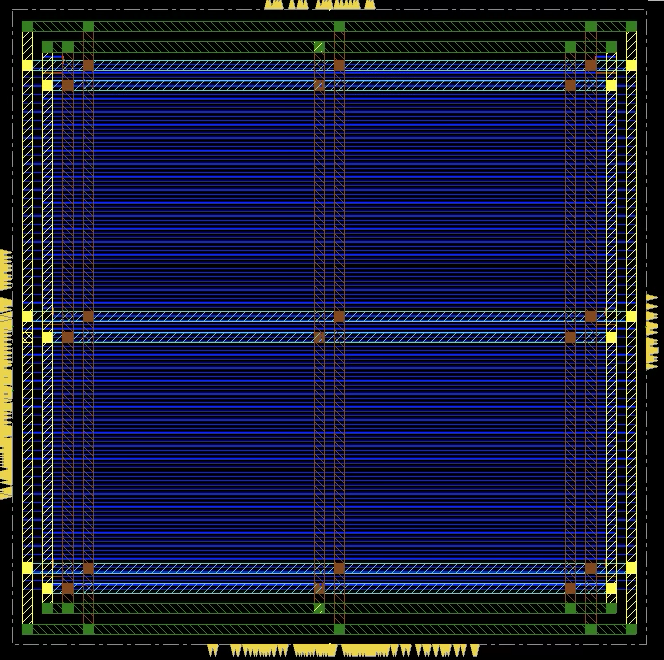
\includegraphics[width=0.8\textwidth]{assets/fig1_1_pdn.png}
    \caption{Power Distribution Network}
\end{figure}

Επόμενο βήμα είναι η τοποθέτηση. Επιλέγεται high effort για τον χρονισμό, καμία βελτιστοποίηση ισχύος και τοποθέτηση των I/O. Όλες οι υπόλοιπες παράμετροι αφήνονται όπως είναι. Παρακάτω ακολουθούν οι πίνακες με τα αποτελέσματα που ζητούνται. Η συνολική επιφάνεια είναι $34284.474~\mu m^2$.

\begin{table}[H]
    \centering
    \caption{Setup Slack for each path type pre Clock Tree Synthesis}
    \begin{tabular}{lr}
        \toprule
        Category & Setup Slack (ns) \\
        \midrule
        I2O & - \\
        I2R & 2.566 \\
        R2O & 3.053 \\
        R2R & 1.444 \\
        \bottomrule
    \end{tabular}
\end{table}

\begin{figure}[H]
    \centering
    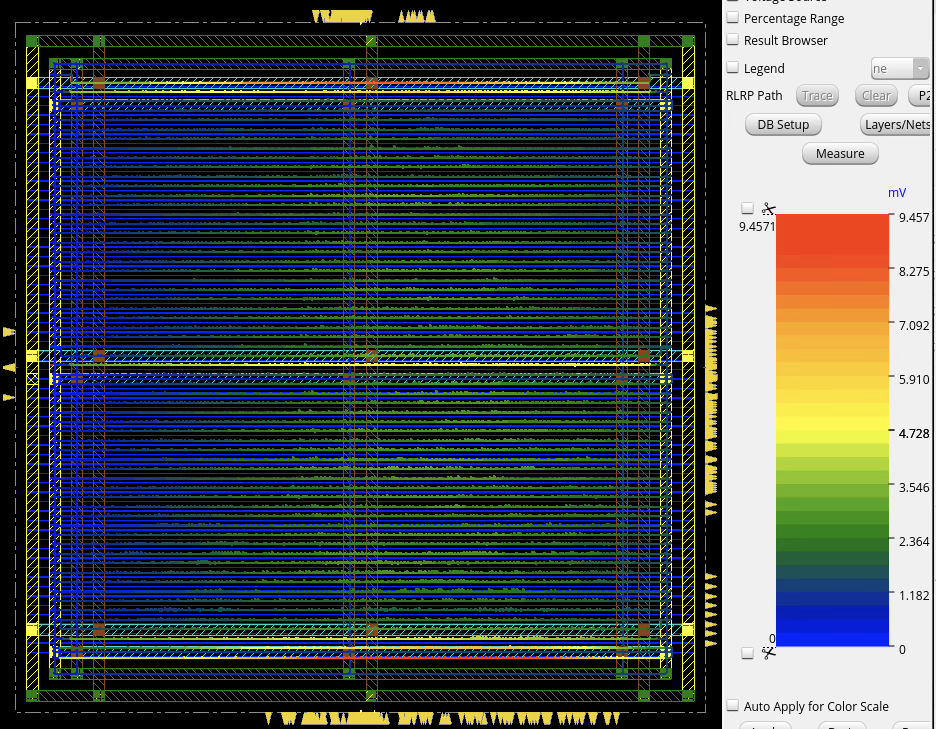
\includegraphics[width=0.8\textwidth]{assets/fig1_2_rail_analysis.png}
    \caption{Results of Early Power Rail Analysis}
\end{figure}

\begin{table}[H]
    \centering
    \caption{Power Consumption per Category pre Clock Tree Synthesis}
    \begin{tabular}{lrrrrr}
        \toprule
        Category & Leakage (mW) & Internal (mW) & Switching (mW) & Total (mW) & Row \% \\
        \midrule
        Sequential & $1.94\times10^{-3}$ & 3.556 & 0.521 & 4.079 & 43.65 \\
        Macro & 0.0 & 0.0 & 0.0 & 0.0 & 0.0 \\
        IO & 0.0 & 0.0 & 0.0 & 0.0 & 0.0 \\
        Combinational & $2.36\times10^{-3}$ & 1.486 & 3.779 & 5.267 & 59.35 \\
        Clock (Comb) & 0.0 & 0.0 & 0.0 & 0.0 & 0.0 \\
        Clock (Seq) & 0.0 & 0.0 & 0.0 & 0.0 & 0.0 \\
        \midrule
        \textbf{Total} & $4.27\times10^{-3}$ & \textbf{5.042} & \textbf{4.3} & \textbf{9.346} & \textbf{100.0} \\
        \bottomrule
    \end{tabular}
\end{table}

Στη συνέχεια γίνεται Early Power Rail ανάλυση. Ακολουθείται η διαδικασία που δίνεται στο εγχειρίδιο εργαστηρίου και προκύπτουν τα παρακάτω αποτελέσματα.

Φαίνεται από το οπτικοποιημένο αποτέλεσμα της ανάλυσης (Figure 1.2) ότι πολλές γραμμές εμφανίζουν πτώση τάσης. Θεωρώ αποδεκτή έως και 7\%, αν και όχι ιδανική. Η μεγαλύτερη πτώση τάσης εμφανίζεται στα rails της άνω και κάτω πλευράς, ρίχνοντας την τάση κατά 9.5 mV. Η τιμή αυτή αντιπροσωπεύει $\frac{9.5}{1320}\approx7.2\%$, ποσοστό οριακά ανεκτό στη συγκεκριμένη υλοποίηση, έτσι ώστε να θεωρείται ότι δεν επηρεάζει την λειτουργία του κυκλώματος. Πιθανότατα, σε εμπορική υλοποίηση να μην είναι αποδεκτό τέτοιο ποσοστό.

Η γραμμή τροφοδοσίας περνάει ακριβώς πάνω από τις περιοχές όπου εμφανίζεται η μεγαλύτερη πτώση τάσης. Αυτό μπορεί να σημαίνει ότι το κύκλωμα είναι πιο “λογικά πυκνό" σε εκείνο το μέρος (Figure 1.3) ή ότι η αντίσταση του grid είναι μεγαλύτερη.

\begin{figure}[H]
    \centering
    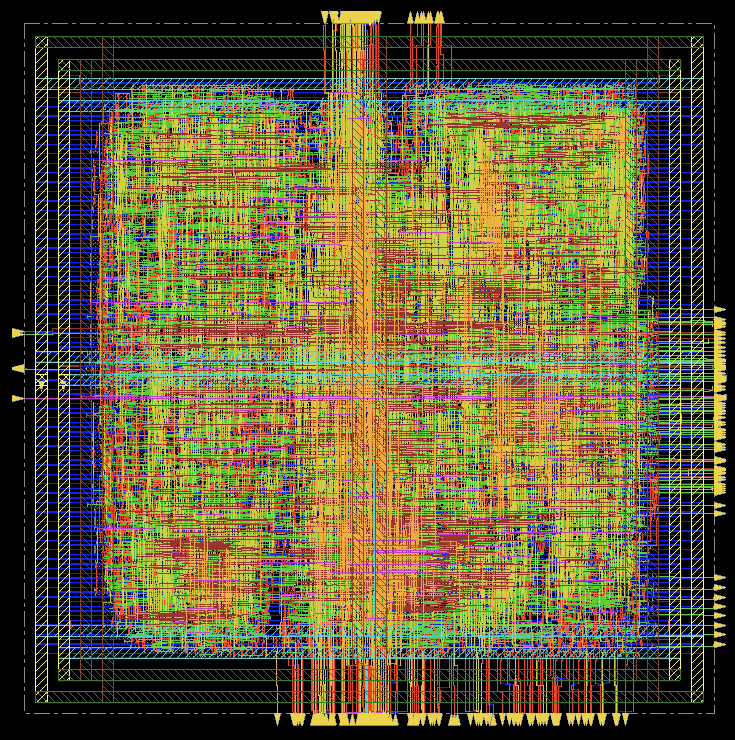
\includegraphics[width=0.8\textwidth]{assets/fig1_3_placement.png}
    \caption{Design Placement}
\end{figure}

Επόμενο στάδιο αποτελεί η Early Global Routing. Στην πρώτη περίπτωση καλύπτονται όλα τα μέταλλα στο εύρος δρομολόγησης (M1-M11) ενώ στη δεύτερη μόνο τα M5-M10. Εκτελώντας την εντολή \texttt{reportCongestion -hotspot} δεν παρατηρείται κάποια διαφοροποίηση: σε καμία περίπτωση δεν ανιχνεύεται συμφόρηση ή hotspot. Παρακάτω παρατίθενται οι πόροι που χρησιμοποιούνται σε καθεμία από τις περιπτώσεις.

\begin{table}[H]
    \centering
    \caption{Resources used for Early Global Routing}
    \begin{tabular}{lrr}
        \toprule
        Metals Used & Wirelength ($\mu m$) & Via (\#) \\
        \midrule
        M1-M11 & 202415.800 & 108727 \\
        M5-M11 & 202180.095 & 229240 \\
        \bottomrule
    \end{tabular}
\end{table}

Παρατηρείται ότι το μήκος των καλωδίων είναι παρόμοιο και στις δυο περιπτώσεις. Ωστόσο, κοιτάζοντας τα στατιστικά είναι εμφανές ότι η πλειοψηφία των καλωδίων θέλει να είναι σε όσο χαμηλότερο επίπεδο γίνεται. Μάλιστα, στην περίπτωση χρήσης των μετάλων M1-M11 τα μήκη στα επίπεδα M6-M11 είναι αμελητέα ενώ στην περίπτωση χρήσης των M5-M10 το ίδιο συμβαίνει στα επίπεδα M9-M10 (<10\%).

Όσον αφορά τα vias, είναι προφανής η διαφορά στο πλήθος που χρησιμοποιούνται. Παρότι το γεγονός ότι η δρομολόγηση των σημάτων περιορίστηκε στα μέταλλα M5-M10 η χρήση via1-via4 παραμένει σημαντική επειδή τα pins των κελιών εξακολουθούν να βρίσκονται στα μέταλλα M1/M2. Ο δρομολογητής πρέπει να δημιουργήσει via stacks για να φτάσει το M5, έχοντας ως αποτέλεσμα πολλαπλά vias χαμηλού επιπέδου χωρίς αντίστοιχο μήκος καλωδίου σε εκείνες τις στρώσεις. Αυτό εξηγεί την $2\times$ κατανάλωση πόρων vias παρά τη μηδενική οριζόντια δρομολόγηση στα χαμηλότερα μέταλλα.

Το επόμενο βήμα αφορά τη σύνθεση του δέντρου ρολογιού. Δημιουργείται ένα NDR με διπλάσιο πάχος και default κενό για όλα τα μέταλλα για το trunk του δέντρου και ο default NDR για τα leaves. Το ελάχιστο και μέγιστο επίπεδο είναι M6 και M7 αντίστοιχα, εφόσον το δίκτυο διανομής χρησιμοποιεί τα μέταλλα M11 έως M8. Τέλος, προστίθεται προστασία και από τις δύο μεριές στο ρολόι χρησιμοποιώντας το VSS net ως shield net, τίθεται 1 ns στρέβλωση και μέγιστος ρυθμός μετάβασης 0.04 ns. Από τη σύνθεση του δέντρου ρολογιού και τη βελτιστοποίηση του κυκλώματος προκύπτουν οι παρακάτω πίνακες.

Η σύνθεση χρησιμοποιεί 24 buffers ρολογιού και κανέναν αντιστροφέα. Στη σχεδίαση υπάρχει μοναδικό skew group. Η στρέβλωση που επιτεύχθηκε είναι 0.012 ns, πολύ μικρότερη από την επιθυμητή ενώ ο επιθυμητός μέγιστος ρυθμός μετάβασης ρολογιού δεν ξεπεράστηκε κατά 0.001 ns (worst transition $= 0.039ns$).

Το μέγιστο και ελάχιστο βάθος του δέντρου ρολογιού ήταν 1, γεγονός που σημαίνει ότι το δέντρο είναι "ρηχό" και κάθε καταχωρητής οδηγείται από ακριβώς έναν buffer (μέσω ενός επιπέδου διανομής). Ένα τόσο ρηχό δέντρο είναι ασυνήθιστο, ωστόσο κρίνεται αποδεκτό στη συγκεκριμένη περίπτωση λόγω του μικρού μεγέθους της σχεδίασης $(250\mu m \times 250\mu m)$, όπου η οδήγηση του σήματος μπορεί να επιτευχθεί αποτελεσματικά χωρίς πολλαπλά επίπεδα επαναληπτών. Το εργαλείο επέλεξε αυτή τη λύση ως τη βέλτιστη για την ικανοποίηση των χρονικών περιορισμών με ελάχιστη χρήση πόρων. Τέλος, το trunk έχει συνολικό μήκος διαδρομής 629.405 $\mu m$ και τα leaves $9072.510~\mu m$.

Ακολουθούν πίνακες με τα αποτελέσματα για setup και hold slack και την κατανάλωση ισχύος. Η συνολική επιφάνεια είναι $34627.842~\mu m^2$.

\begin{table}[H]
    \centering
    \caption{Setup and Hold Slack post Clock Tree Synthesis}
    \begin{tabular}{lrr}
        \toprule
        Category & Setup Slack (ns) & Hold Slack (ns) \\
        \midrule
        I2O & - & - \\
        I2R & 2.519 & 0.240 \\
        R2O & 3.052 & 0.296 \\
        R2R & 1.413 & 0.033 \\
        \bottomrule
    \end{tabular}
\end{table}

\begin{table}[H]
    \centering
    \caption{Power Consumption per Category post Clock Tree Synthesis}
    \begin{tabular}{lrrrrr}
        \toprule
        Category & Leakage (mW) & Internal (mW) & Switching (mW) & Total (mW) & Row \% \\
        \midrule
        Sequential & $1.93\times10^{-3}$ & 3.535 & 0.46 & 3.997 & 38.14 \\
        Macro & 0.0 & 0.0 & 0.0 & 0.0 & 0.0 \\
        IO & 0.0 & 0.0 & 0.0 & 0.0 & 0.0 \\
        Combinational & $2.38\times10^{-3}$ & 1.515 & 3.899 & 5.416 & 51.68 \\
        Clock (Comb) & $4.81\times10^{-5}$ & 0.232 & 0.8352 & 1.067 & 10.19 \\
        Clock (Seq) & 0.0 & 0.0 & 0.0 & 0.0 & 0.0 \\
        \midrule
        \textbf{Total} & $4.36\times10^{-3}$ & \textbf{5.283} & \textbf{5.194} & \textbf{10.48} & \textbf{100.0} \\
        \bottomrule
    \end{tabular}
\end{table}

Έπειτα ακολουθεί η δρομολόγηση. Επιλέγονται οι ρυθμίσεις Fix Antenna, SI Driven, Timing Driven με effort 5, Via Optimization με medium effort όπως ορίζει η εκφώνηση και παρακάτω βρίσκονται τα αποτελέσματα.
Ακολουθούν πίνακες με τα αποτελέσματα για setup και hold slack και την κατανάλωση ισχύος. Η συνολική επιφάνεια είναι $34627.842~\mu m^2$.

\begin{table}[H]
    \centering
    \caption{Setup and Hold Slack post Routing}
    \begin{tabular}{lrr}
        \toprule
        Category & Setup Slack (ns) & Hold Slack (ns) \\
        \midrule
        I2O & - & - \\
        I2R & 2.531 & 0.241 \\
        R2O & 3.054 & 0.295 \\
        R2R & 1.452 & 0.032 \\
        \bottomrule
    \end{tabular}
\end{table}

\begin{table}[H]
    \centering
    \caption{Power Consumption per Category post Routing}
    \begin{tabular}{lrrrrr}
        \toprule
        Category & Leakage (mW) & Internal (mW) & Switching (mW) & Total (mW) & Row \% \\
        \midrule
        Sequential & $1.93\times10^{-3}$ & 3.537 & 0.452 & 3.991 & 38.15 \\
        Macro & 0.0 & 0.0 & 0.0 & 0.0 & 0.0 \\
        IO & 0.0 & 0.0 & 0.0 & 0.0 & 0.0 \\
        Combinational & $2.38\times10^{-3}$ & 1.513 & 3.863 & 5.379 & 51.43 \\
        Clock (Comb) & $4.81\times10^{-5}$ & 0.232 & 0.858 & 1.09 & 10.42 \\
        Clock (Seq) & 0.0 & 0.0 & 0.0 & 0.0 & 0.0 \\
        \midrule
        \textbf{Total} & $4.355\times10^{-3}$ & \textbf{5.283} & \textbf{5.173} & \textbf{10.46} & \textbf{100} \\
        \bottomrule
    \end{tabular}
\end{table}

Τέλος, ελέγχεται το φυσικό σχέδιο για DRC παραβιάσεις μέσω της εντολής \texttt{verify drc}. Στη συνέχεια προστίθενται Fillers σε όλα τα επίπεδα με ελάχιστο όριο πυκνότητας το 10\% για όλα τα μέταλλα.

Εμφανίστηκαν DRC παραβάσεις οι οποίες δεν λύθηκαν με την εκτέλεση της εντολής \texttt{ecoroute -fix\_drc} και παρατίθενται παρακάτω.
\begin{itemize}
    \item Metal Short
    \item Metal Spacing
    \item End-of-Line Spacing
\end{itemize}
\newpage

\section{Άσκηση 2}
Η βασική διαφοροποίηση μεταξύ των δύο ασκήσεων έγκειται στη στρατηγική σύνθεσης που ακολουθήθηκε στο εργαλείο Genus. Ενώ στην Άσκηση 1 τηρήθηκε η προεπιλεγμένη ροή με πρωταρχικό στόχο την ικανοποίηση των χρονικών περιορισμών (timing), στην Άσκηση 2 ενεργοποιήθηκαν ρητά εντολές βελτιστοποίησης ισχύος (\texttt{design\_power\_effort high}) με αποκλειστική στόχευση τη δυναμική ισχύ (\texttt{opt\_leakage\_to\_dynamic\_ratio 0.0}). Η αλλαγή αυτή μετέβαλε τη συνάρτηση κόστους του αλγορίθμου, αναγκάζοντας το εργαλείο να προβεί σε δομικές αλλαγές και επιλογή ενεργειακά αποδοτικότερων πυλών, θυσιάζοντας ενδεχομένως μέρος της επιφάνειας ή του πλεονάζοντος χρονισμού.

\begin{table}[H]
    \centering
    \caption{Total number of cells of each type post Synthesis}
    \begin{tabular}{lrrrrrr}
        \toprule
         & \multicolumn{3}{c}{\textbf{Άσκηση 1}} & \multicolumn{3}{c}{\textbf{Άσκηση 2}} \\
        \cmidrule(lr){2-4} \cmidrule(lr){5-7}
        Type & Instances & Area ($\mu m^2$) & Area \% & Instances & Area ($\mu m^2$) & Area \% \\
        \midrule
        Sequential & 2399 & 18048.366 & 52.8 & 2399 & 15073.992 & 42.8 \\
        Inverter & 238 & 165.870 & 0.5 & 411 & 292.068 & 0.8 \\
        Buffer & 27 & 97.470 & 0.3 & 16 & 49.932 & 0.1 \\
        Logic & 6994 & 15865.722 & 46.4 & 8159 & 19844.550 & 56.3 \\
        \midrule
        \textbf{Total} & \textbf{9658} & \textbf{34177.428} & \textbf{100.0} & \textbf{10985} & \textbf{35260.542} & \textbf{100.0} \\
        \bottomrule
    \end{tabular}
\end{table}

\begin{table}[H]
    \centering
    \caption{Power consumption per category post Synthesis}
    \resizebox{\textwidth}{!}{
    \begin{tabular}{lrrrrrrrrrr}
        \toprule
         & \multicolumn{5}{c}{\textbf{Άσκηση 1}} & \multicolumn{5}{c}{\textbf{Άσκηση 2}} \\
        \cmidrule(lr){2-6} \cmidrule(lr){7-11}
        Category & Leakage (mW) & Internal (mW) & Switching (mW) & Total (mW) & Row \% & Leakage (mW) & Internal (mW) & Switching (mW) & Total (mW) & Row \% \\
        \midrule
        Register & $2.06\times10^{-3}$ & 4.04 & 3.21 & 7.26 & 66.30\% & $1.66\times10^{-3}$ & 2.8 & 2.88 & 5.68 & 68.20\% \\
        Logic & $2.20\times10^{-3}$ & 1.10 & 2.31 & 3.40 & 33.70\% & $2.05\times10^{-3}$ & 0.9 & 1.74 & 2.65 & 31.8\% \\
        Subtotal & $4.26\times10^{-3}$ & 5.14 & 5.52 & 10.07 & 100.0\% & $3.72\times10^{-3}$ & 3.7 & 4.63 & 8.33 & 100.0\% \\
        Percentage & 0.04\% & 48.21\% & 51.75\% & 100.0\% & & 0.04\% & 44.41\% & 55.54\% & 100\% & \\
        \bottomrule
    \end{tabular}}
\end{table}

\begin{table}[H]
    \centering
    \caption{Slack for each path type post Synthesis}
    \begin{tabular}{lrr}
        \toprule
        Category & Άσκηση 1 Slack (ns) & Άσκηση 2 Slack (ns) \\
        \midrule
        I2O & - & - \\
        I2R & 2.141 & 2.193 \\
        R2O & 3.125 & 3.051 \\
        R2R & 0.994 & 0.986 \\
        \bottomrule
    \end{tabular}
\end{table}

\begin{table}[H]
    \centering
    \caption{Total Area pre Clock Tree Synthesis}
    \begin{tabular}{lr}
        \toprule
        Category & Area ($\mu m^2$) \\
        \midrule
        Άσκηση 1 & 34284.474 \\
        Άσκηση 2 & 34783.794 \\
        \bottomrule
    \end{tabular}
\end{table}

\begin{table}[H]
    \centering
    \caption{Setup Slack for each path type pre Clock Tree Synthesis}
    \begin{tabular}{lrr}
        \toprule
        Category & Άσκηση 1 Setup Slack (ns) & Άσκηση 2 Setup Slack (ns) \\
        \midrule
        I2O & - & - \\
        I2R & 2.566 & 2.601 \\
        R2O & 3.053 & 2.998 \\
        R2R & 1.444 & 1.349 \\
        \bottomrule
    \end{tabular}
\end{table}

\begin{table}[H]
    \centering
    \caption{Power Consumption per Category pre Clock Tree Synthesis}
    \resizebox{\textwidth}{!}{
    \begin{tabular}{lrrrrrrrrrr}
        \toprule
         & \multicolumn{5}{c}{\textbf{Άσκηση 1}} & \multicolumn{5}{c}{\textbf{Άσκηση 2}} \\
        \cmidrule(lr){2-6} \cmidrule(lr){7-11}
        Category & Leakage (mW) & Internal (mW) & Switching (mW) & Total (mW) & Row \% & Leakage (mW) & Internal (mW) & Switching (mW) & Total (mW) & Row \% \\
        \midrule
        Sequential & $1.94\times10^{-3}$ & 3.556 & 0.521 & 4.079 & 43.65 & $1.44\times10^{-3}$ & 2.736 & 0.289 & 3.026 & 36.45 \\
        Combinational & $2.36\times10^{-3}$ & 1.486 & 3.779 & 5.267 & 59.35 & $2.26\times10^{-3}$ & 1.322 & 3.951 & 5.275 & 63.55 \\
        Total & $4.27\times10^{-3}$ & 5.042 & 4.3 & 9.346 & 100.0 & $3.7\times10^{-3}$ & 4.059 & 4.239 & 8.302 & 100.0 \\
        \bottomrule
    \end{tabular}}
\end{table}

\begin{table}[H]
    \centering
    \caption{Total area post Clock Tree Synthesis}
    \begin{tabular}{lr}
        \toprule
        Category & Area ($\mu m^2$) \\
        \midrule
        Άσκηση 1 & 34627.842 \\
        Άσκηση 2 & 34953.084 \\
        \bottomrule
    \end{tabular}
\end{table}

\begin{table}[H]
    \centering
    \caption{Setup and Hold Slack post Clock Tree Synthesis}
    \begin{tabular}{lrrrr}
        \toprule
         & \multicolumn{2}{c}{\textbf{Άσκηση 1}} & \multicolumn{2}{c}{\textbf{Άσκηση 2}} \\
        \cmidrule(lr){2-3} \cmidrule(lr){4-5}
        Category & Setup Slack (ns) & Hold Slack (ns) & Setup Slack (ns) & Hold Slack (ns) \\
        \midrule
        I2O & - & - & - & - \\
        I2R & 2.519 & 0.240 & 2.595 & 0.248 \\
        R2O & 3.052 & 0.296 & 2.996 & 0.302 \\
        R2R & 1.413 & 0.033 & 1.336 & 0.030 \\
        \bottomrule
    \end{tabular}
\end{table}

\begin{table}[H]
    \centering
    \caption{Power Consumption per Category post Clock Tree Synthesis}
    \resizebox{\textwidth}{!}{
    \begin{tabular}{lrrrrrrrrrr}
        \toprule
         & \multicolumn{5}{c}{\textbf{Άσκηση 1}} & \multicolumn{5}{c}{\textbf{Άσκηση 2}} \\
        \cmidrule(lr){2-6} \cmidrule(lr){7-11}
        Category & Leakage (mW) & Internal (mW) & Switching (mW) & Total (mW) & Row \% & Leakage (mW) & Internal (mW) & Switching (mW) & Total (mW) & Row \% \\
        \midrule
        Sequential & $1.93\times10^{-3}$ & 3.535 & 0.46 & 3.997 & 38.14 & $1.44\times10^{-3}$ & 2.723 & 0.291 & 3.015 & 32.27 \\
        Combinational & $2.38\times10^{-3}$ & 1.515 & 3.899 & 5.416 & 51.68 & $2.26\times10^{-3}$ & 1.322 & 3.953 & 5.277 & 56.48 \\
        Clock (Comb) & $4.81\times10^{-5}$ & 0.232 & 0.8352 & 1.067 & 10.19 & $4.59\times10^{-5}$ & 0.2192 & 0.832 & 1.052 & 11.25 \\
        Total & $4.36\times10^{-3}$ & 5.283 & 5.194 & 10.48 & 100.0 & $3.75\times10^{-3}$ & 4.264 & 5.076 & 9.344 & 100 \\
        \bottomrule
    \end{tabular}}
\end{table}

\begin{table}[H]
    \centering
    \caption{Total Area post Routing}
    \begin{tabular}{lr}
        \toprule
        Category & Area ($\mu m^2$) \\
        \midrule
        Άσκηση 1 & 34627.842 \\
        Άσκηση 2 & 34953.084 \\
        \bottomrule
    \end{tabular}
\end{table}

\begin{table}[H]
    \centering
    \caption{Setup and Hold Slack post Routing}
    \begin{tabular}{lrrrr}
        \toprule
         & \multicolumn{2}{c}{\textbf{Άσκηση 1}} & \multicolumn{2}{c}{\textbf{Άσκηση 2}} \\
        \cmidrule(lr){2-3} \cmidrule(lr){4-5}
        Category & Setup Slack (ns) & Hold Slack (ns) & Setup Slack (ns) & Hold Slack (ns) \\
        \midrule
        I2O & - & - & - & - \\
        I2R & 2.531 & 0.241 & 2.573 & 0.249 \\
        R2O & 3.054 & 0.295 & 2.992 & 0.301 \\
        R2R & 1.452 & 0.032 & 1.363 & 0.031 \\
        \bottomrule
    \end{tabular}
\end{table}

\begin{table}[H]
    \centering
    \caption{Power Consumption per Category post Routing}
    \resizebox{\textwidth}{!}{
    \begin{tabular}{lrrrrrrrrrr}
        \toprule
         & \multicolumn{5}{c}{\textbf{Άσκηση 1}} & \multicolumn{5}{c}{\textbf{Άσκηση 2}} \\
        \cmidrule(lr){2-6} \cmidrule(lr){7-11}
        Category & Leakage (mW) & Internal (mW) & Switching (mW) & Total (mW) & Row \% & Leakage (mW) & Internal (mW) & Switching (mW) & Total (mW) & Row \% \\
        \midrule
        Sequential & $1.93\times10^{-3}$ & 3.537 & 0.452 & 3.991 & 38.15 & $1.44\times10^{-3}$ & 2.717 & 0.267 & 2.986 & 32.87 \\
        Combinational & $2.38\times10^{-3}$ & 1.513 & 3.863 & 5.379 & 51.43 & $2.26\times10^{-3}$ & 1.311 & 3.796 & 5.109 & 56.23 \\
        Clock (Comb) & $4.81\times10^{-5}$ & 0.232 & 0.858 & 1.09 & 10.42 & $4.59\times10^{-5}$ & 0.2191 & 0.7715 & 0.991 & 10.9 \\
        Total & $4.355\times10^{-3}$ & 5.283 & 5.173 & 10.46 & 100 & $3.75\times10^{-3}$ & 4.246 & 4.835 & 9.086 & 100 \\
        \bottomrule
    \end{tabular}}
\end{table}

Τα συγκεντρωτικά δεδομένα των πινάκων καταδεικνύουν την επιτυχή εφαρμογή της βελτιστοποίησης, η οποία επέφερε σημαντική μείωση της συνολικής κατανάλωσης ισχύος κατά 17,3\% (από 10,07 mW σε 8,33 mW) στο στάδιο Post-Synthesis, η οποία διατηρήθηκε και μετά τη δρομολόγηση (Post-Routing) με τελική μείωση 13,1\% (από 10,46 mW σε 9,086 mW). Η μείωση προήλθε σχεδόν αποκλειστικά από τον περιορισμό της δυναμικής ισχύος (Switching \& Internal). 

Ως αντιστάθμισμα (trade-off) για αυτήν την ενεργειακή βελτίωση, παρατηρείται αφενός μια μικρή αύξηση της τάξης του 3\% στην επιφάνεια και το πλήθος των κελιών -γεγονός που υποδηλώνει αναδιάρθρωση της λογικής για μείωση της δραστηριότητας μεταγωγής και αφετέρου μια αναμενόμενη, μικρή μείωση στα χρονικά περιθώρια (Slack), τα οποία ωστόσο παρέμειναν θετικά, διασφαλίζοντας την ορθή λειτουργία του κυκλώματος.
\newpage

\section{Άσκηση 3}
Στην Άσκηση 3, ο σχεδιαστικός στόχος μετατοπίστηκε στη μεγιστοποίηση της απόδοσης, αυξάνοντας τη συχνότητα λειτουργίας στα 400 MHz (περίοδος ρολογιού 2,5 ns) σε σύγκριση με τα 250 MHz (4,0 ns) της Άσκησης 1. Για την υλοποίηση αυτής της αλλαγής, τροποποιήθηκαν οι χρονικοί περιορισμοί στο αρχείο SDC (περίοδος και μέγιστος ρυθμός μετάβασης), ενώ η στρατηγική σύνθεσης στο Genus επανήλθε στην τυπική βελτιστοποίηση με γνώμονα τον χρονισμό (timing-driven), χωρίς τις εξειδικευμένες εντολές χαμηλής ισχύος που χρησιμοποιήθηκαν στην Άσκηση 2.

\begin{table}[H]
    \centering
    \caption{Total number of cells of each type post Synthesis}
    \begin{tabular}{lrrrrrr}
        \toprule
         & \multicolumn{3}{c}{\textbf{Άσκηση 1}} & \multicolumn{3}{c}{\textbf{Άσκηση 3}} \\
        \cmidrule(lr){2-4} \cmidrule(lr){5-7}
        Type & Instances & Area ($\mu m^2$) & Area \% & Instances & Area ($\mu m^2$) & Area \% \\
        \midrule
        Sequential & 2399 & 18048.366 & 52.8 & 2399 & 18032.634 & 51.6 \\
        Inverter & 238 & 165.870 & 0.5 & 270 & 188.100 & 0.5 \\
        Buffer & 27 & 97.470 & 0.3 & 28 & 101.232 & 0.3 \\
        Logic & 6994 & 15865.722 & 46.4 & 7351 & 16620.858 & 47.6 \\
        \midrule
        \textbf{Total} & \textbf{9658} & \textbf{34177.428} & \textbf{100.0} & \textbf{10048} & \textbf{34942.824} & \textbf{100.0} \\
        \bottomrule
    \end{tabular}
\end{table}

\begin{table}[H]
    \centering
    \caption{Power consumption per category post Synthesis}
    \resizebox{\textwidth}{!}{
    \begin{tabular}{lrrrrrrrrrr}
        \toprule
         & \multicolumn{5}{c}{\textbf{Άσκηση 1}} & \multicolumn{5}{c}{\textbf{Άσκηση 3}} \\
        \cmidrule(lr){2-6} \cmidrule(lr){7-11}
        Category & Leakage (mW) & Internal (mW) & Switching (mW) & Total (mW) & Row \% & Leakage (mW) & Internal (mW) & Switching (mW) & Total (mW) & Row \% \\
        \midrule
        Register & $2.06\times10^{-3}$ & 4.04 & 3.21 & 7.26 & 66.30\% & $2.05\times10^{-3}$ & 6.36 & 5.09 & 11.46 & 67.54\% \\
        Logic & $2.20\times10^{-3}$ & 1.10 & 2.31 & 3.40 & 33.70\% & $2.30\times10^{-3}$ & 1.73 & 3.77 & 5.51 & 32.46\% \\
        Subtotal & $4.26\times10^{-3}$ & 5.14 & 5.52 & 10.07 & 100.0\% & $4.35\times10^{-3}$ & 8.09 & 8.87 & 17.00 & 100.0\% \\
        Percentage & 0.04\% & 48.21\% & 51.75\% & 100.0\% & & 0.03\% & 47.70\% & 52.72\% & 100.0\% & \\
        \bottomrule
    \end{tabular}}
\end{table}

\begin{table}[H]
    \centering
    \caption{Slack for each path type post Synthesis}
    \begin{tabular}{lrr}
        \toprule
        Category & Άσκηση 1 Slack (ns) & Άσκηση 3 Slack (ns) \\
        \midrule
        I2O & - & - \\
        I2R & 2.141 & 0.646 \\
        R2O & 3.125 & 1.627 \\
        R2R & 0.994 & 0.007 \\
        \bottomrule
    \end{tabular}
\end{table}

\begin{table}[H]
    \centering
    \caption{Total Area pre Clock Tree Synthesis}
    \begin{tabular}{lr}
        \toprule
        Category & Area ($\mu m^2$) \\
        \midrule
        Άσκηση 1 & 34284.474 \\
        Άσκηση 3 & 35061.156 \\
        \bottomrule
    \end{tabular}
\end{table}

\begin{table}[H]
    \centering
    \caption{Setup Slack for each path type pre Clock Tree Synthesis}
    \begin{tabular}{lrr}
        \toprule
        Category & Άσκηση 1 Setup Slack (ns) & Άσκηση 3 Setup Slack (ns) \\
        \midrule
        I2O & - & - \\
        I2R & 2.566 & 0.985 \\
        R2O & 3.053 & 1.614 \\
        R2R & 1.444 & 0.531 \\
        \bottomrule
    \end{tabular}
\end{table}

\begin{table}[H]
    \centering
    \caption{Power Consumption per Category pre Clock Tree Synthesis}
    \resizebox{\textwidth}{!}{
    \begin{tabular}{lrrrrrrrrrr}
        \toprule
         & \multicolumn{5}{c}{\textbf{Άσκηση 1}} & \multicolumn{5}{c}{\textbf{Άσκηση 3}} \\
        \cmidrule(lr){2-6} \cmidrule(lr){7-11}
        Category & Leakage (mW) & Internal (mW) & Switching (mW) & Total (mW) & Row \% & Leakage (mW) & Internal (mW) & Switching (mW) & Total (mW) & Row \% \\
        \midrule
        Sequential & $1.94\times10^{-3}$ & 3.556 & 0.521 & 4.079 & 43.65 & $1.94\times10^{-3}$ & 5.601 & 0.841 & 6.444 & 45.71 \\
        Combinational & $2.36\times10^{-3}$ & 1.486 & 3.779 & 5.267 & 59.35 & $2.43\times10^{-3}$ & 1.941 & 5.709 & 7.652 & 54.29 \\
        Total & $4.27\times10^{-3}$ & 5.042 & 4.3 & 9.346 & 100.0 & $4.37\times10^{-3}$ & 7.542 & 6.549 & 14.1 & 100.0 \\
        \bottomrule
    \end{tabular}}
\end{table}

\begin{table}[H]
    \centering
    \caption{Total area post Clock Tree Synthesis}
    \begin{tabular}{lr}
        \toprule
        Category & Area ($\mu m^2$) \\
        \midrule
        Άσκηση 1 & 34627.842 \\
        Άσκηση 3 & 35316.972 \\
        \bottomrule
    \end{tabular}
\end{table}

\begin{table}[H]
    \centering
    \caption{Setup and Hold Slack post Clock Tree Synthesis}
    \begin{tabular}{lrrrr}
        \toprule
         & \multicolumn{2}{c}{\textbf{Άσκηση 1}} & \multicolumn{2}{c}{\textbf{Άσκηση 3}} \\
        \cmidrule(lr){2-3} \cmidrule(lr){4-5}
        Category & Setup Slack (ns) & Hold Slack (ns) & Setup Slack (ns) & Hold Slack (ns) \\
        \midrule
        I2O & - & - & - & - \\
        I2R & 2.519 & 0.240 & 0.981 & 0.244 \\
        R2O & 3.052 & 0.296 & 1.621 & 0.295 \\
        R2R & 1.413 & 0.033 & 0.530 & 0.033 \\
        \bottomrule
    \end{tabular}
\end{table}

\begin{table}[H]
    \centering
    \caption{Power Consumption per Category post Clock Tree Synthesis}
    \resizebox{\textwidth}{!}{
    \begin{tabular}{lrrrrrrrrrr}
        \toprule
         & \multicolumn{5}{c}{\textbf{Άσκηση 1}} & \multicolumn{5}{c}{\textbf{Άσκηση 3}} \\
        \cmidrule(lr){2-6} \cmidrule(lr){7-11}
        Category & Leakage (mW) & Internal (mW) & Switching (mW) & Total (mW) & Row \% & Leakage (mW) & Internal (mW) & Switching (mW) & Total (mW) & Row \% \\
        \midrule
        Sequential & $1.93\times10^{-3}$ & 3.535 & 0.46 & 3.997 & 38.14 & $1.92\times10^{-3}$ & 5.581 & 0.845 & 6.428 & 39.53 \\
        Combinational & $2.38\times10^{-3}$ & 1.515 & 3.899 & 5.416 & 51.68 & $2.43\times10^{-3}$ & 1.943 & 5.71 & 7.655 & 47.08 \\
        Clock (Comb) & $4.81\times10^{-5}$ & 0.232 & 0.8352 & 1.067 & 10.19 & $9.11\times10^{-5}$ & 0.720 & 1.456 & 2.177 & 13.39 \\
        Total & $4.36\times10^{-3}$ & 5.283 & 5.194 & 10.48 & 100.0 & $4.44\times10^{-3}$ & 8.244 & 8.011 & 16.26 & 100 \\
        \bottomrule
    \end{tabular}}
\end{table}

\begin{table}[H]
    \centering
    \caption{Total Area post Routing}
    \begin{tabular}{lr}
        \toprule
        Category & Area ($\mu m^2$) \\
        \midrule
        Άσκηση 1 & 34627.842 \\
        Άσκηση 3 & 35316.972 \\
        \bottomrule
    \end{tabular}
\end{table}

\begin{table}[H]
    \centering
    \caption{Setup and Hold Slack post Routing}
    \begin{tabular}{lrrrr}
        \toprule
         & \multicolumn{2}{c}{\textbf{Άσκηση 1}} & \multicolumn{2}{c}{\textbf{Άσκηση 3}} \\
        \cmidrule(lr){2-3} \cmidrule(lr){4-5}
        Category & Setup Slack (ns) & Hold Slack (ns) & Setup Slack (ns) & Hold Slack (ns) \\
        \midrule
        I2O & - & - & - & - \\
        I2R & 2.531 & 0.241 & 0.968 & 0.245 \\
        R2O & 3.054 & 0.295 & 1.615 & 0.294 \\
        R2R & 1.452 & 0.032 & 0.501 & 0.032 \\
        \bottomrule
    \end{tabular}
\end{table}

\begin{table}[H]
    \centering
    \caption{Power Consumption per Category post Routing}
    \resizebox{\textwidth}{!}{
    \begin{tabular}{lrrrrrrrrrr}
        \toprule
         & \multicolumn{5}{c}{\textbf{Άσκηση 1}} & \multicolumn{5}{c}{\textbf{Άσκηση 3}} \\
        \cmidrule(lr){2-6} \cmidrule(lr){7-11}
        Category & Leakage (mW) & Internal (mW) & Switching (mW) & Total (mW) & Row \% & Leakage (mW) & Internal (mW) & Switching (mW) & Total (mW) & Row \% \\
        \midrule
        Sequential & $1.93\times10^{-3}$ & 3.537 & 0.452 & 3.991 & 38.15 & $1.92\times10^{-3}$ & 5.572 & 0.797 & 6.371 & 40.14 \\
        Combinational & $2.38\times10^{-3}$ & 1.513 & 3.863 & 5.379 & 51.43 & $2.43\times10^{-3}$ & 1.926 & 5.503 & 7.432 & 46.82 \\
        Clock (Comb) & $4.81\times10^{-5}$ & 0.232 & 0.858 & 1.09 & 10.42 & $9.11\times10^{-5}$ & 0.72 & 1.349 & 2.069 & 13.04 \\
        Total & $4.355\times10^{-3}$ & 5.283 & 5.173 & 10.46 & 100 & $4.44\times10^{-3}$ & 8.218 & 7.65 & 15.87 & 100 \\
        \bottomrule
    \end{tabular}}
\end{table}

Τα αποτελέσματα αναδεικνύουν το κόστος της υψηλής ταχύτητας, με κυριότερο χαρακτηριστικό τη δραματική αύξηση της συνολικής κατανάλωσης ισχύος κατά περίπου 69\% (από 10,07 mW σε 17,00 mW) στο στάδιο Post-Synthesis και 51,7\% (από 10,46 mW σε 15,87 mW) μετά τη δρομολόγηση, ακολουθώντας την αναλογική σχέση συχνότητας και δυναμικής ισχύος. 

Η προσπάθεια του εργαλείου να ικανοποιήσει τους αυστηρούς χρονικούς περιορισμούς οδήγησε σε μικρή αύξηση της επιφάνειας και του πλήθους των πυλών, ενώ το Setup Slack συρρικνώθηκε σημαντικά (φτάνοντας τα 0,007 ns Post-Synthesis και 0,501 ns Post-Routing), υποδεικνύοντας ότι το κύκλωμα λειτουργεί πλέον κοντά στα όρια των δυνατοτήτων του για τη συγκεκριμένη τεχνολογία.
\newpage

\section{Άσκηση 4}
Στην Άσκηση 4, η ροή σχεδίασης παραμένει δομικά πανομοιότυπη με την Άσκηση 1, διατηρώντας τους ίδιους χρονικούς περιορισμούς (250 MHz) και την ίδια τυπική στρατηγική σύνθεσης. Η ειδοποιός διαφορά εντοπίζεται στην αντικατάσταση της βιβλιοθήκης χρονισμού \texttt{fast\_vdd1v2} (Best-Case PVT) με την \texttt{slow\_vdd1v2} (Worst-Case PVT), προσομοιώνοντας τη λειτουργία του κυκλώματος υπό δυσμενείς συνθήκες (χαμηλότερη τάση 1.08V, υψηλότερη θερμοκρασία, αργή διαδικασία κατασκευής), επιβάλλοντας στο εργαλείο να διαχειριστεί αυξημένες καθυστερήσεις για να επιτύχει το κλείσιμο των χρονισμών.

\begin{table}[H]
    \centering
    \caption{Total number of cells of each type post Synthesis}
    \begin{tabular}{lrrrrrr}
        \toprule
         & \multicolumn{3}{c}{\textbf{Άσκηση 1}} & \multicolumn{3}{c}{\textbf{Άσκηση 4}} \\
        \cmidrule(lr){2-4} \cmidrule(lr){5-7}
        Type & Instances & Area ($\mu m^2$) & Area \% & Instances & Area ($\mu m^2$) & Area \% \\
        \midrule
        Sequential & 2399 & 18048.366 & 52.8 & 2398 & 17489.196 & 46.8 \\
        Inverter & 238 & 165.870 & 0.5 & 325 & 252.054 & 0.7 \\
        Buffer & 27 & 97.470 & 0.3 & 250 & 1730.520 & 4.6 \\
        Logic & 6994 & 15865.722 & 46.4 & 8072 & 17895.834 & 47.9 \\
        \midrule
        \textbf{Total} & \textbf{9658} & \textbf{34177.428} & \textbf{100.0} & \textbf{11045} & \textbf{37367.604} & \textbf{100.0} \\
        \bottomrule
    \end{tabular}
\end{table}

\begin{table}[H]
    \centering
    \caption{Power consumption per category post Synthesis}
    \resizebox{\textwidth}{!}{
    \begin{tabular}{lrrrrrrrrrr}
        \toprule
         & \multicolumn{5}{c}{\textbf{Άσκηση 1}} & \multicolumn{5}{c}{\textbf{Άσκηση 4}} \\
        \cmidrule(lr){2-6} \cmidrule(lr){7-11}
        Category & Leakage (mW) & Internal (mW) & Switching (mW) & Total (mW) & Row \% & Leakage (mW) & Internal (mW) & Switching (mW) & Total (mW) & Row \% \\
        \midrule
        Register & $2.06\times10^{-3}$ & 4.04 & 3.21 & 7.26 & 66.30\% & $0.53\times10^{-3}$ & 2.10 & 0.25 & 2.36 & 39.38\% \\
        Logic & $2.20\times10^{-3}$ & 1.10 & 2.31 & 3.40 & 33.70\% & $0.88\times10^{-3}$ & 7.69 & 2.86 & 3.63 & 60.62\% \\
        Subtotal & $4.26\times10^{-3}$ & 5.14 & 5.52 & 10.07 & 100.0\% & $1.42\times10^{-3}$ & 2.87 & 3.11 & 5.98 & 100.0\% \\
        Percentage & 0.04\% & 48.21\% & 51.75\% & 100.0\% & & 0.02\% & 48.02\% & 51.95\% & 100\% & \\
        \bottomrule
    \end{tabular}}
\end{table}

\begin{table}[H]
    \centering
    \caption{Slack for each path type post Synthesis}
    \begin{tabular}{lrr}
        \toprule
        Category & Άσκηση 1 Slack (ns) & Άσκηση 4 Slack (ns) \\
        \midrule
        I2O & - & - \\
        I2R & 2.141 & 1.384 \\
        R2O & 3.125 & 2.790 \\
        R2R & 0.994 & 0.00 \\
        \bottomrule
    \end{tabular}
\end{table}

\begin{table}[H]
    \centering
    \caption{Total Area pre Clock Tree Synthesis}
    \begin{tabular}{lr}
        \toprule
        Category & Area ($\mu m^2$) \\
        \midrule
        Άσκηση 1 & 34284.474 \\
        Άσκηση 4 & 37450.710 \\
        \bottomrule
    \end{tabular}
\end{table}

\begin{table}[H]
    \centering
    \caption{Setup Slack for each path type pre Clock Tree Synthesis}
    \begin{tabular}{lrr}
        \toprule
        Category & Άσκηση 1 Setup Slack (ns) & Άσκηση 4 Setup Slack (ns) \\
        \midrule
        I2O & - & - \\
        I2R & 2.566 & 1.615 \\
        R2O & 3.053 & 2.631 \\
        R2R & 1.444 & 0.094 \\
        \bottomrule
    \end{tabular}
\end{table}

\begin{table}[H]
    \centering
    \caption{Power Consumption per Category pre Clock Tree Synthesis}
    \resizebox{\textwidth}{!}{
    \begin{tabular}{lrrrrrrrrrr}
        \toprule
         & \multicolumn{5}{c}{\textbf{Άσκηση 1}} & \multicolumn{5}{c}{\textbf{Άσκηση 4}} \\
        \cmidrule(lr){2-6} \cmidrule(lr){7-11}
        Category & Leakage (mW) & Internal (mW) & Switching (mW) & Total (mW) & Row \% & Leakage (mW) & Internal (mW) & Switching (mW) & Total (mW) & Row \% \\
        \midrule
        Sequential & $1.94\times10^{-3}$ & 3.556 & 0.521 & 4.079 & 43.65 & $0.53\times10^{-3}$ & 2.155 & 0.21 & 2.365 & 40.8 \\
        Combinational & $2.36\times10^{-3}$ & 1.486 & 3.779 & 5.267 & 59.35 & $0.89\times10^{-3}$ & 0.933 & 2.498 & 3.432 & 59.2 \\
        Total & $4.27\times10^{-3}$ & 5.042 & 4.3 & 9.346 & 100.0 & $1.42\times10^{-3}$ & 3.087 & 2.707 & 5.796 & 100.0 \\
        \bottomrule
    \end{tabular}}
\end{table}

\begin{table}[H]
    \centering
    \caption{Total area post Clock Tree Synthesis}
    \begin{tabular}{lr}
        \toprule
        Category & Area ($\mu m^2$) \\
        \midrule
        Άσκηση 1 & 34627.842 \\
        Άσκηση 4 & 37939.770 \\
        \bottomrule
    \end{tabular}
\end{table}

\begin{table}[H]
    \centering
    \caption{Setup and Hold Slack post Clock Tree Synthesis}
    \begin{tabular}{lrrrr}
        \toprule
         & \multicolumn{2}{c}{\textbf{Άσκηση 1}} & \multicolumn{2}{c}{\textbf{Άσκηση 4}} \\
        \cmidrule(lr){2-3} \cmidrule(lr){4-5}
        Category & Setup Slack (ns) & Hold Slack (ns) & Setup Slack (ns) & Hold Slack (ns) \\
        \midrule
        I2O & - & - & - & - \\
        I2R & 2.519 & 0.240 & 1.586 & 0.258 \\
        R2O & 3.052 & 0.296 & 2.629 & 0.429 \\
        R2R & 1.413 & 0.033 & 0.066 & 0.121 \\
        \bottomrule
    \end{tabular}
\end{table}

\begin{table}[H]
    \centering
    \caption{Power Consumption per Category post Clock Tree Synthesis}
    \resizebox{\textwidth}{!}{
    \begin{tabular}{lrrrrrrrrrr}
        \toprule
         & \multicolumn{5}{c}{\textbf{Άσκηση 1}} & \multicolumn{5}{c}{\textbf{Άσκηση 4}} \\
        \cmidrule(lr){2-6} \cmidrule(lr){7-11}
        Category & Leakage (mW) & Internal (mW) & Switching (mW) & Total (mW) & Row \% & Leakage (mW) & Internal (mW) & Switching (mW) & Total (mW) & Row \% \\
        \midrule
        Sequential & $1.93\times10^{-3}$ & 3.535 & 0.46 & 3.997 & 38.14 & $0.53\times10^{-3}$ & 2.154 & 0.2135 & 2.368 & 35.1 \\
        Combinational & $2.38\times10^{-3}$ & 1.515 & 3.899 & 5.416 & 51.68 & $0.89\times10^{-3}$ & 0.934 & 2.511 & 3.445 & 51.06 \\
        Clock (Comb) & $4.81\times10^{-5}$ & 0.232 & 0.8352 & 1.067 & 10.19 & $0.06\times10^{-3}$ & 0.3771 & 0.557 & 0.934 & 13.85 \\
        Total & $4.36\times10^{-3}$ & 5.283 & 5.194 & 10.48 & 100.0 & $1.48\times10^{-3}$ & 3.465 & 3.281 & 6.748 & 100 \\
        \bottomrule
    \end{tabular}}
\end{table}

Πρέπει να σημειωθεί ότι το εργαλείο δεν επέτρεπε τη χρήση του χρόνου μετάβασης του ρολογιού στα 0.04 ns (1\% της περιόδου όπως ορίζει η εκφώνηση) λόγω περιορισμών στις βιβλιοθήκες lef, οπότε χρησιμοποιήθηκε χρόνος μετάβασης ρολογιού 0.045 ns (1.125\% της περιόδου ρολογιού).

\begin{table}[H]
    \centering
    \caption{Total Area post Routing}
    \begin{tabular}{lr}
        \toprule
        Category & Area ($\mu m^2$) \\
        \midrule
        Άσκηση 1 & 34627.842 \\
        Άσκηση 4 & 37939.770 \\
        \bottomrule
    \end{tabular}
\end{table}

\begin{table}[H]
    \centering
    \caption{Setup and Hold Slack post Routing}
    \begin{tabular}{lrrrr}
        \toprule
         & \multicolumn{2}{c}{\textbf{Άσκηση 1}} & \multicolumn{2}{c}{\textbf{Άσκηση 4}} \\
        \cmidrule(lr){2-3} \cmidrule(lr){4-5}
        Category & Setup Slack (ns) & Hold Slack (ns) & Setup Slack (ns) & Hold Slack (ns) \\
        \midrule
        I2O & - & - & - & - \\
        I2R & 2.531 & 0.241 & 1.499 & 0.256 \\
        R2O & 3.054 & 0.295 & 2.661 & 0.428 \\
        R2R & 1.452 & 0.032 & 0.065 & 0.113 \\
        \bottomrule
    \end{tabular}
\end{table}

\begin{table}[H]
    \centering
    \caption{Power Consumption per Category post Routing}
    \resizebox{\textwidth}{!}{
    \begin{tabular}{lrrrrrrrrrr}
        \toprule
         & \multicolumn{5}{c}{\textbf{Άσκηση 1}} & \multicolumn{5}{c}{\textbf{Άσκηση 4}} \\
        \cmidrule(lr){2-6} \cmidrule(lr){7-11}
        Category & Leakage (mW) & Internal (mW) & Switching (mW) & Total (mW) & Row \% & Leakage (mW) & Internal (mW) & Switching (mW) & Total (mW) & Row \% \\
        \midrule
        Sequential & $1.93\times10^{-3}$ & 3.537 & 0.452 & 3.991 & 38.15 & $0.53\times10^{-3}$ & 2.154 & 0.1995 & 2.354 & 35.34 \\
        Combinational & $2.38\times10^{-3}$ & 1.513 & 3.863 & 5.379 & 51.43 & $0.89\times10^{-3}$ & 0.935 & 2.445 & 3.381 & 50.75 \\
        Clock (Comb) & $4.81\times10^{-5}$ & 0.232 & 0.858 & 1.09 & 10.42 & $5.51\times10^{-3}$ & 0.3772 & 0.549 & 0.927 & 13.91 \\
        Total & $4.355\times10^{-3}$ & 5.283 & 5.173 & 10.46 & 100 & $1.48\times10^{-3}$ & 3.466 & 3.194 & 6.662 & 100 \\
        \bottomrule
    \end{tabular}}
\end{table}

Η μετάβαση στη slow βιβλιοθήκη ανάγκασε το εργαλείο σύνθεσης να αντισταθμίσει τη μειωμένη ταχύτητα των πυλών αυξάνοντας δραστικά τον αριθμό των buffers (από 27 σε 250) και τη συνολική επιφάνεια κατά $\approx$9.3\% Post-Synthesis και $\approx$9.6\% Post-Routing. Παρά την αύξηση του υλικού, η συνολική κατανάλωση ισχύος μειώθηκε εντυπωσιακά κατά $\approx$36-40\% σε όλα τα στάδια, γεγονός που οφείλεται στη χαμηλότερη τάση λειτουργίας (1.08V έναντι 1.32V), η οποία επηρεάζει τετραγωνικά τη δυναμική ισχύ. Το Setup Slack περιορίστηκε οριακά (φτάνοντας τα 0,00 ns Post-Synthesis και 0,065 ns Post-Routing), δείχνοντας ότι το κύκλωμα εξάντλησε τα χρονικά περιθώρια για να ικανοποιήσει τους περιορισμούς υπό τις χειρότερες συνθήκες λειτουργίας.
\newpage

\section{Άσκηση 5}
Στην Άσκηση 5, εφαρμόστηκε η τεχνική της φραγής ρολογιού (Clock Gating) με στόχο τη δραστική μείωση της δυναμικής κατανάλωσης ισχύος, διατηρώντας τις παραμέτρους της βασικής υλοποίησης (Task 1: 250 MHz, Fast Library). Η διαδικασία ενεργοποιήθηκε στο εργαλείο Genus μέσω της εντολής \texttt{set\_db lp\_insert\_clock\_gating true} πριν από το στάδιο του elaboration, επιτρέποντας στον αλγόριθμο σύνθεσης να εντοπίσει αυτόματα τις ομάδες καταχωρητών που μπορούν να μοιραστούν ένα κοινό σήμα ενεργοποίησης και να προσθέσει ειδικά κελιά ICG (Integrated Clock Gating) στο δέντρο του ρολογιού.

\begin{table}[H]
    \centering
    \caption{Total number of cells of each type post Synthesis}
    \begin{tabular}{lrrrrrr}
        \toprule
         & \multicolumn{3}{c}{\textbf{Άσκηση 1}} & \multicolumn{3}{c}{\textbf{Άσκηση 5}} \\
        \cmidrule(lr){2-4} \cmidrule(lr){5-7}
        Type & Instances & Area ($\mu m^2$) & Area \% & Instances & Area ($\mu m^2$) & Area \% \\
        \midrule
        Sequential & 2399 & 18048.366 & 52.8 & 2398 & 14214.546 & 48.2 \\
        Inverter & 238 & 165.870 & 0.5 & 239 & 167.238 & 0.6 \\
        Buffer & 27 & 97.470 & 0.3 & 7 & 19.494 & 0.1 \\
        Logic & 6994 & 15865.722 & 46.4 & 6508 & 14725.494 & 49.9 \\
        Clock Gating Integrated Cell & - & - & - & 60 & 389.880 & 1.3 \\
        \midrule
        \textbf{Total} & \textbf{9658} & \textbf{34177.428} & \textbf{100.0} & \textbf{9212} & \textbf{29516.652} & \textbf{100.0} \\
        \bottomrule
    \end{tabular}
\end{table}

\begin{table}[H]
    \centering
    \caption{Power consumption per category post Synthesis}
    \resizebox{\textwidth}{!}{
    \begin{tabular}{lrrrrrrrrrr}
        \toprule
         & \multicolumn{5}{c}{\textbf{Άσκηση 1}} & \multicolumn{5}{c}{\textbf{Άσκηση 5}} \\
        \cmidrule(lr){2-6} \cmidrule(lr){7-11}
        Category & Leakage (mW) & Internal (mW) & Switching (mW) & Total (mW) & Row \% & Leakage (mW) & Internal (mW) & Switching (mW) & Total (mW) & Row \% \\
        \midrule
        Register & $2.06\times10^{-3}$ & 4.04 & 3.21 & 7.26 & 66.30\% & $1.9\times10^{-3}$ & 1.7 & 2.50 & 4.21 & 74.95\% \\
        Logic & $2.20\times10^{-3}$ & 1.10 & 2.31 & 3.40 & 33.70\% & $2.06\times10^{-3}$ & 0.44 & 0.79 & 1.23 & 21.83\% \\
        Clock & 0.0 & 0.0 & 0.0 & 0.0 & 0.0\% & $4.06\times10^{-5}$ & 0.08 & 0.1 & 0.18 & 3.22\% \\
        Subtotal & $4.26\times10^{-3}$ & 5.14 & 5.52 & 10.07 & 100.0\% & $4\times10^{-3}$ & 2.23 & 3.38 & 5.61 & 100.0\% \\
        Percentage & 0.04\% & 48.21\% & 51.75\% & 100.0\% & & 0.07\% & 39.73\% & 60.2\% & 100\% & \\
        \bottomrule
    \end{tabular}}
\end{table}

\begin{table}[H]
    \centering
    \caption{Slack for each path type post Synthesis}
    \begin{tabular}{lrr}
        \toprule
        Category & Άσκηση 1 Slack (ns) & Άσκηση 5 Slack (ns) \\
        \midrule
        I2O & - & - \\
        I2R & 2.141 & 2.606 \\
        R2O & 3.125 & 3.125 \\
        R2R & 0.994 & 1.033 \\
        \bottomrule
    \end{tabular}
\end{table}

\begin{table}[H]
    \centering
    \caption{Clock Gating Use Statistics}
    \begin{tabular}{lrrr}
        \toprule
        Category & Number & Percentage & Average Toggle Saving \% \\
        \midrule
        Total Clock Gating Instances & 60 & 100.00 & - \\
        RC Clock Gating Instances & 60 & 100.00 & 83.39 \\
        RC Gated Flip-Flops & 2013 & 83.94 & 85.07 \\
        Total Gated Flip-Flops & 2013 & 83.94 & - \\
        Total Ungated Flip-Flops & 385 & 16.06 & - \\
        Enable not found & 336 & 87.27 & - \\
        Register bank width too small & 49 & 12.73 & - \\
        Total Flip-Flops & 2398 & 100.00 & - \\
        \bottomrule
    \end{tabular}
\end{table}

\begin{table}[H]
    \centering
    \caption{Total Area pre Clock Tree Synthesis}
    \begin{tabular}{lr}
        \toprule
        Category & Area ($\mu m^2$) \\
        \midrule
        Άσκηση 1 & 34284.474 \\
        Άσκηση 5 & 29616.858 \\
        \bottomrule
    \end{tabular}
\end{table}

\begin{table}[H]
    \centering
    \caption{Setup Slack for each path type pre Clock Tree Synthesis}
    \begin{tabular}{lrr}
        \toprule
        Category & Άσκηση 1 Setup Slack (ns) & Άσκηση 5 Setup Slack (ns) \\
        \midrule
        I2O & - & - \\
        I2R & 2.566 & 2.700 \\
        R2O & 3.053 & 3.081 \\
        R2R & 1.444 & 1.428 \\
        \bottomrule
    \end{tabular}
\end{table}

\begin{table}[H]
    \centering
    \caption{Power Consumption per Category pre Clock Tree Synthesis}
    \resizebox{\textwidth}{!}{
    \begin{tabular}{lrrrrrrrrrr}
        \toprule
         & \multicolumn{5}{c}{\textbf{Άσκηση 1}} & \multicolumn{5}{c}{\textbf{Άσκηση 5}} \\
        \cmidrule(lr){2-6} \cmidrule(lr){7-11}
        Category & Leakage (mW) & Internal (mW) & Switching (mW) & Total (mW) & Row \% & Leakage (mW) & Internal (mW) & Switching (mW) & Total (mW) & Row \% \\
        \midrule
        Sequential & $1.94\times10^{-3}$ & 3.556 & 0.521 & 4.079 & 43.65 & $1.77\times10^{-3}$ & 1.744 & 0.746 & 2.492 & 32.96 \\
        Combinational & $2.36\times10^{-3}$ & 1.486 & 3.779 & 5.267 & 59.35 & $2.2\times10^{-3}$ & 1.44 & 3.536 & 4.978 & 65.84 \\
        Clock (Sequential) & - & - & - & - & - & $4.06\times10^{-5}$ & 0.091 & 0 & 0.091 & 1.204 \\
        Total & $4.27\times10^{-3}$ & 5.042 & 4.3 & 9.346 & 100.0 & $4.01\times10^{-3}$ & 3.275 & 4.283 & 7.561 & 100.0 \\
        \bottomrule
    \end{tabular}}
\end{table}

\begin{table}[H]
    \centering
    \caption{Total area post Clock Tree Synthesis}
    \begin{tabular}{lr}
        \toprule
        Category & Area ($\mu m^2$) \\
        \midrule
        Άσκηση 1 & 34627.842 \\
        Άσκηση 5 & 29770.416 \\
        \bottomrule
    \end{tabular}
\end{table}

\begin{table}[H]
    \centering
    \caption{Setup and Hold Slack post Clock Tree Synthesis}
    \begin{tabular}{lrrrr}
        \toprule
         & \multicolumn{2}{c}{\textbf{Άσκηση 1}} & \multicolumn{2}{c}{\textbf{Άσκηση 5}} \\
        \cmidrule(lr){2-3} \cmidrule(lr){4-5}
        Category & Setup Slack (ns) & Hold Slack (ns) & Setup Slack (ns) & Hold Slack (ns) \\
        \midrule
        I2O & - & - & - & - \\
        I2R & 2.519 & 0.240 & 2.688 & 0.238 \\
        R2O & 3.052 & 0.296 & 3.092 & 0.286 \\
        R2R & 1.413 & 0.033 & 0.006 & 1.404 \\
        \bottomrule
    \end{tabular}
\end{table}

\begin{table}[H]
    \centering
    \caption{Power Consumption per Category post Clock Tree Synthesis}
    \resizebox{\textwidth}{!}{
    \begin{tabular}{lrrrrrrrrrr}
        \toprule
         & \multicolumn{5}{c}{\textbf{Άσκηση 1}} & \multicolumn{5}{c}{\textbf{Άσκηση 5}} \\
        \cmidrule(lr){2-6} \cmidrule(lr){7-11}
        Category & Leakage (mW) & Internal (mW) & Switching (mW) & Total (mW) & Row \% & Leakage (mW) & Internal (mW) & Switching (mW) & Total (mW) & Row \% \\
        \midrule
        Sequential & $1.93\times10^{-3}$ & 3.535 & 0.46 & 3.997 & 38.14 & $1.77\times10^{-3}$ & 1.737 & 0.749 & 2.488 & 31.05 \\
        Combinational & $2.38\times10^{-3}$ & 1.515 & 3.899 & 5.416 & 51.68 & $2.2\times10^{-3}$ & 1.44 & 3.533 & 4.976 & 62.11 \\
        Clock (Comb) & $4.81\times10^{-5}$ & 0.232 & 0.8352 & 1.067 & 10.19 & $0.008\times10^{-3}$ & 0.038 & 0.1484 & 0.1866 & 2.329 \\
        Clock (Sequential) & - & - & - & - & - & $0.08\times10^{-3}$ & 0.206 & 0.1553 & 0.361 & 4.51 \\
        Total & $4.36\times10^{-3}$ & 5.283 & 5.194 & 10.48 & 100.0 & $4.1\times10^{-3}$ & 3.422 & 4.586 & 8.011 & 100 \\
        \bottomrule
    \end{tabular}}
\end{table}

\begin{table}[H]
    \centering
    \caption{Total Area post Routing}
    \begin{tabular}{lr}
        \toprule
        Category & Area ($\mu m^2$) \\
        \midrule
        Άσκηση 1 & 34627.842 \\
        Άσκηση 5 & 29770.416 \\
        \bottomrule
    \end{tabular}
\end{table}

\begin{table}[H]
    \centering
    \caption{Setup and Hold Slack post Routing}
    \begin{tabular}{lrrrr}
        \toprule
         & \multicolumn{2}{c}{\textbf{Άσκηση 1}} & \multicolumn{2}{c}{\textbf{Άσκηση 5}} \\
        \cmidrule(lr){2-3} \cmidrule(lr){4-5}
        Category & Setup Slack (ns) & Hold Slack (ns) & Setup Slack (ns) & Hold Slack (ns) \\
        \midrule
        I2O & - & - & - & - \\
        I2R & 2.531 & 0.241 & 2.671 & 0.238 \\
        R2O & 3.054 & 0.295 & 3.090 & 0.285 \\
        R2R & 1.452 & 0.032 & 1.410 & 0.005 \\
        \bottomrule
    \end{tabular}
\end{table}

\begin{table}[H]
    \centering
    \caption{Power Consumption per Category post Routing}
    \resizebox{\textwidth}{!}{
    \begin{tabular}{lrrrrrrrrrr}
        \toprule
         & \multicolumn{5}{c}{\textbf{Άσκηση 1}} & \multicolumn{5}{c}{\textbf{Άσκηση 5}} \\
        \cmidrule(lr){2-6} \cmidrule(lr){7-11}
        Category & Leakage (mW) & Internal (mW) & Switching (mW) & Total (mW) & Row \% & Leakage (mW) & Internal (mW) & Switching (mW) & Total (mW) & Row \% \\
        \midrule
        Sequential & $1.93\times10^{-3}$ & 3.537 & 0.452 & 3.991 & 38.15 & $1.77\times10^{-3}$ & 1.733 & 0.7216 & 2.456 & 31.37 \\
        Combinational & $2.38\times10^{-3}$ & 1.513 & 3.863 & 5.379 & 51.43 & $2.2\times10^{-3}$ & 1.432 & 3.41 & 4.844 & 61.87 \\
        Clock (Comb) & $4.81\times10^{-5}$ & 0.232 & 0.858 & 1.09 & 10.42 & $8\times10^{-6}$ & 0.038 & 0.1396 & 0.1778 & 2.271 \\
        Clock (Sequential) & - & - & - & - & - & $8\times10^{-5}$ & 0.206 & 0.146 & 0.3519 & 4.495 \\
        Total & $4.355\times10^{-3}$ & 5.283 & 5.173 & 10.46 & 100 & $4.1\times10^{-3}$ & 3.409 & 4.417 & 7.83 & 100 \\
        \bottomrule
    \end{tabular}}
\end{table}

Τα στατιστικά στοιχεία δείχνουν ότι η εφαρμογή της τεχνικής ήταν ιδιαίτερα επιτυχής, με την εισαγωγή 60 κελιών ICG που οδήγησαν στη φραγή του 83,94\% των συνολικών flip-flops. Η επίδραση αυτή αποτυπώνεται ξεκάθαρα στα αποτελέσματα μετά τη δρομολόγηση, όπου η συνολική κατανάλωση ισχύος μειώθηκε κατά 25,1\% (από 10,46 mW σε 7,83 mW), κυρίως λόγω του περιορισμού της κατανάλωσης του δικτύου ρολογιού και της Internal Power. Επιπλέον, η επιφάνεια μειώθηκε εντυπωσιακά κατά $\approx$14\% (από $34.627~\mu m^2$ σε $29.770~\mu m^2$), πιθανώς λόγω της αφαίρεσης των πολυπλεκτών επανατροφοδότησης που αντικαταστάθηκαν από τη λογική clock gating, ενώ το Setup Slack παρέμεινε σε εξαιρετικά επίπεδα, αποδεικνύοντας ότι η εξοικονόμηση ενέργειας δεν επιβάρυνε την απόδοση.
\newpage

\section{Άσκηση 6}
Στην Άσκηση 6, ο στόχος ήταν η ενσωμάτωση υποδομής ελέγχου (DFT) μέσω της τεχνικής Scan Chain Insertion, όπου τα συμβατικά flip-flops αντικαταστάθηκαν από Scan Flip-Flops (SDFF) που σχηματίζουν μια ενιαία αλυσίδα σάρωσης. Η βασική διαφορά από την Άσκηση 1 είναι η χρήση των εντολών DFT στο Genus (\texttt{connect\_scan\_chains}, \texttt{write\_scandef}) και η ανάγνωση του αρχείου \texttt{.scandef} στο Innovus (\texttt{defIn}), επιτρέποντας στο εργαλείο φυσικής σχεδίασης να αναγνωρίσει την αλυσίδα και να βελτιστοποιήσει τη σειρά σύνδεσης των καταχωρητών (Scan Reordering) για τη μείωση του μήκους καλωδίωσης.

\begin{table}[H]
    \centering
    \caption{Total number of cells of each type post Synthesis}
    \begin{tabular}{lrrrrrr}
        \toprule
         & \multicolumn{3}{c}{\textbf{Άσκηση 1}} & \multicolumn{3}{c}{\textbf{Άσκηση 6}} \\
        \cmidrule(lr){2-4} \cmidrule(lr){5-7}
        Type & Instances & Area ($\mu m^2$) & Area \% & Instances & Area ($\mu m^2$) & Area \% \\
        \midrule
        Sequential & 2399 & 18048.366 & 52.8 & 2399 & 18800.424 & 49.3 \\
        Inverter & 238 & 165.870 & 0.5 & 366 & 253.422 & 0.7 \\
        Buffer & 27 & 97.470 & 0.3 & 5 & 14.706 & 0.0 \\
        Logic & 6994 & 15865.722 & 46.4 & 8331 & 19062.396 & 50.0 \\
        \midrule
        \textbf{Total} & \textbf{9658} & \textbf{34177.428} & \textbf{100.0} & \textbf{11101} & \textbf{38130.948} & \textbf{100.0} \\
        \bottomrule
    \end{tabular}
\end{table}

\begin{table}[H]
    \centering
    \caption{Power consumption per category post Synthesis}
    \resizebox{\textwidth}{!}{
    \begin{tabular}{lrrrrrrrrrr}
        \toprule
         & \multicolumn{5}{c}{\textbf{Άσκηση 1}} & \multicolumn{5}{c}{\textbf{Άσκηση 6}} \\
        \cmidrule(lr){2-6} \cmidrule(lr){7-11}
        Category & Leakage (mW) & Internal (mW) & Switching (mW) & Total (mW) & Row \% & Leakage (mW) & Internal (mW) & Switching (mW) & Total (mW) & Row \% \\
        \midrule
        Register & $2.06\times10^{-3}$ & 4.04 & 3.21 & 7.26 & 66.30\% & $2.01\times10^{-3}$ & 3.27 & 3.54 & 6.82 & 69.34\% \\
        Logic & $2.20\times10^{-3}$ & 1.10 & 2.31 & 3.40 & 33.70\% & $2.6\times10^{-3}$ & 1.25 & 1.76 & 3.01 & 30.66\% \\
        Subtotal & $4.26\times10^{-3}$ & 5.14 & 5.52 & 10.07 & 100.0\% & $4.65\times10^{-3}$ & 4.52 & 5.3 & 9.83 & 100.0\% \\
        Percentage & 0.04\% & 48.21\% & 51.75\% & 100.0\% & & 0.05\% & 46.03\% & 53.92\% & 100\% & \\
        \bottomrule
    \end{tabular}}
\end{table}

\begin{table}[H]
    \centering
    \caption{Slack for each path type post Synthesis}
    \begin{tabular}{lrr}
        \toprule
        Category & Άσκηση 1 Slack (ns) & Άσκηση 6 Slack (ns) \\
        \midrule
        I2O & - & - \\
        I2R & 2.141 & 2.134 \\
        R2O & 3.125 & 3.124 \\
        R2R & 0.994 & 0.979 \\
        \bottomrule
    \end{tabular}
\end{table}

\begin{table}[H]
    \centering
    \caption{Total Area pre Clock Tree Synthesis}
    \begin{tabular}{lr}
        \toprule
        Category & Area ($\mu m^2$) \\
        \midrule
        Άσκηση 1 & 34284.474 \\
        Άσκηση 6 & 38281.428 \\
        \bottomrule
    \end{tabular}
\end{table}

\begin{table}[H]
    \centering
    \caption{Setup Slack for each path type pre Clock Tree Synthesis}
    \begin{tabular}{lrr}
        \toprule
        Category & Άσκηση 1 Setup Slack (ns) & Άσκηση 6 Setup Slack (ns) \\
        \midrule
        I2O & - & - \\
        I2R & 2.566 & 2.700 \\
        R2O & 3.053 & 3.081 \\
        R2R & 1.444 & 1.428 \\
        \bottomrule
    \end{tabular}
\end{table}

\begin{table}[H]
    \centering
    \caption{Power Consumption per Category pre Clock Tree Synthesis}
    \resizebox{\textwidth}{!}{
    \begin{tabular}{lrrrrrrrrrr}
        \toprule
         & \multicolumn{5}{c}{\textbf{Άσκηση 1}} & \multicolumn{5}{c}{\textbf{Άσκηση 6}} \\
        \cmidrule(lr){2-6} \cmidrule(lr){7-11}
        Category & Leakage (mW) & Internal (mW) & Switching (mW) & Total (mW) & Row \% & Leakage (mW) & Internal (mW) & Switching (mW) & Total (mW) & Row \% \\
        \midrule
        Sequential & $1.94\times10^{-3}$ & 3.556 & 0.521 & 4.079 & 43.65 & $1.9\times10^{-3}$ & 3.535 & 0.473 & 4.01 & 41.14 \\
        Combinational & $2.36\times10^{-3}$ & 1.486 & 3.779 & 5.267 & 59.35 & $2.8\times10^{-3}$ & 1.639 & 4.096 & 5.738 & 58.86 \\
        Total & $4.27\times10^{-3}$ & 5.042 & 4.3 & 9.346 & 100.0 & $4.6\times10^{-3}$ & 5.174 & 4.569 & 9.748 & 100.0 \\
        \bottomrule
    \end{tabular}}
\end{table}

\begin{table}[H]
    \centering
    \caption{Total area post Clock Tree Synthesis}
    \begin{tabular}{lr}
        \toprule
        Category & Area ($\mu m^2$) \\
        \midrule
        Άσκηση 1 & 34627.842 \\
        Άσκηση 6 & 38424.726 \\
        \bottomrule
    \end{tabular}
\end{table}

\begin{table}[H]
    \centering
    \caption{Setup and Hold Slack post Clock Tree Synthesis}
    \begin{tabular}{lrrrr}
        \toprule
         & \multicolumn{2}{c}{\textbf{Άσκηση 1}} & \multicolumn{2}{c}{\textbf{Άσκηση 6}} \\
        \cmidrule(lr){2-3} \cmidrule(lr){4-5}
        Category & Setup Slack (ns) & Hold Slack (ns) & Setup Slack (ns) & Hold Slack (ns) \\
        \midrule
        I2O & - & - & - & - \\
        I2R & 2.519 & 0.240 & 2.443 & -0.011 \\
        R2O & 3.052 & 0.296 & 2.954 & 0.305 \\
        R2R & 1.413 & 0.033 & 1.391 & 0.033 \\
        \bottomrule
    \end{tabular}
\end{table}

\begin{table}[H]
    \centering
    \caption{Power Consumption per Category post Clock Tree Synthesis}
    \resizebox{\textwidth}{!}{
    \begin{tabular}{lrrrrrrrrrr}
        \toprule
         & \multicolumn{5}{c}{\textbf{Άσκηση 1}} & \multicolumn{5}{c}{\textbf{Άσκηση 6}} \\
        \cmidrule(lr){2-6} \cmidrule(lr){7-11}
        Category & Leakage (mW) & Internal (mW) & Switching (mW) & Total (mW) & Row \% & Leakage (mW) & Internal (mW) & Switching (mW) & Total (mW) & Row \% \\
        \midrule
        Sequential & $1.93\times10^{-3}$ & 3.535 & 0.46 & 3.997 & 38.14 & $1.8\times10^{-3}$ & 3.52 & 0.4417 & 3.957 & 37.5 \\
        Combinational & $2.38\times10^{-3}$ & 1.515 & 3.899 & 5.416 & 51.68 & $2.8\times10^{-3}$ & 1.63 & 3.933 & 5.566 & 52.74 \\
        Clock (Comb) & $4.81\times10^{-5}$ & 0.232 & 0.8352 & 1.067 & 10.19 & $0.005\times10^{-3}$ & 0.214 & 0.8161 & 1.03 & 9.761 \\
        Total & $4.36\times10^{-3}$ & 5.283 & 5.194 & 10.48 & 100.0 & $4.7\times10^{-3}$ & 5.358 & 5.191 & 10.55 & 100 \\
        \bottomrule
    \end{tabular}}
\end{table}

\begin{table}[H]
    \centering
    \caption{Total Area post Routing}
    \begin{tabular}{lr}
        \toprule
        Category & Area ($\mu m^2$) \\
        \midrule
        Άσκηση 1 & 34627.842 \\
        Άσκηση 6 & 38424.726 \\
        \bottomrule
    \end{tabular}
\end{table}

\begin{table}[H]
    \centering
    \caption{Setup and Hold Slack post Routing}
    \begin{tabular}{lrrrr}
        \toprule
         & \multicolumn{2}{c}{\textbf{Άσκηση 1}} & \multicolumn{2}{c}{\textbf{Άσκηση 6}} \\
        \cmidrule(lr){2-3} \cmidrule(lr){4-5}
        Category & Setup Slack (ns) & Hold Slack (ns) & Setup Slack (ns) & Hold Slack (ns) \\
        \midrule
        I2O & - & - & - & - \\
        I2R & 2.531 & 0.241 & 2.389 & -0.012 \\
        R2O & 3.054 & 0.295 & 2.949 & 0.305 \\
        R2R & 1.452 & 0.032 & 1.395 & 0.033 \\
        \bottomrule
    \end{tabular}
\end{table}

\begin{table}[H]
    \centering
    \caption{Power Consumption per Category post Routing}
    \resizebox{\textwidth}{!}{
    \begin{tabular}{lrrrrrrrrrr}
        \toprule
         & \multicolumn{5}{c}{\textbf{Άσκηση 1}} & \multicolumn{5}{c}{\textbf{Άσκηση 6}} \\
        \cmidrule(lr){2-6} \cmidrule(lr){7-11}
        Category & Leakage (mW) & Internal (mW) & Switching (mW) & Total (mW) & Row \% & Leakage (mW) & Internal (mW) & Switching (mW) & Total (mW) & Row \% \\
        \midrule
        Sequential & $1.93\times10^{-3}$ & 3.537 & 0.452 & 3.991 & 38.15 & $1.8\times10^{-3}$ & 3.514 & 0.4417 & 3.957 & 37.5 \\
        Combinational & $2.38\times10^{-3}$ & 1.513 & 3.863 & 5.379 & 51.43 & $2.8\times10^{-3}$ & 1.63 & 3.933 & 5.566 & 52.74 \\
        Clock (Comb) & $4.81\times10^{-5}$ & 0.232 & 0.858 & 1.09 & 10.42 & $4.5\times10^{-5}$ & 0.214 & 0.8161 & 1.03 & 9.761 \\
        Total & $4.355\times10^{-3}$ & 5.283 & 5.173 & 10.46 & 100 & $4.7\times10^{-3}$ & 5.358 & 5.191 & 10.55 & 100 \\
        \bottomrule
    \end{tabular}}
\end{table}

\begin{table}[H]
    \centering
    \caption{Scan Chain Information}
    \begin{tabular}{lr}
        \toprule
        Category & \# \\
        \midrule
        Scan Bits & 2399 \\
        Float Wire Length & 17975.270 \\
        Order Wire Length & 281.550 \\
        Total Wire Length & 18256.820 \\
        \bottomrule
    \end{tabular}
\end{table}

Η επίδραση του DFT είναι εμφανής στην αύξηση της συνολικής επιφάνειας του κυκλώματος κατά $\approx$11\% (από 34627 $\mu m^2$ σε 38424 $\mu m^2$ Post-Routing), η οποία οφείλεται στη χρήση των μεγαλύτερων κελιών SDFF που περιλαμβάνουν πολυπλέκτη εισόδου. Η κατανάλωση ισχύος παρουσίασε μικρή αύξηση (από 10.46 mW σε 10.55 mW Post-Routing), πιθανώς λόγω βελτιστοποιήσεων στη λογική, ενώ το Setup Slack μειώθηκε ελαφρώς (από 1.452 ns σε 1.395 ns) λόγω της πρόσθετης καθυστέρησης των SDFFS. Η επιτυχία της διαδικασίας επιβεβαιώνεται από την αναφορά της αλυσίδας σάρωσης (2399 bits, Status VALID) και τη δραστική μείωση του μήκους καλωδίωσης της αλυσίδας κατά $\approx$98\% μέσω του Scan Reordering στο Innovus.
\newpage

\section{Άσκηση 7}
Στην Άσκηση 7, πραγματοποιήθηκε τυπική επαλήθευση (Formal Verification) χρησιμοποιώντας το εργαλείο Conformal LEC για να επιβεβαιωθεί η λογική ακεραιότητα της σχεδίασης κατά τη διαδικασία της σύνθεσης. Εκτελέστηκαν δύο συγκρίσεις: αρχικά συγκρίθηκε ο κώδικας RTL με το στιγμιότυπο του elaboration (RTL vs Elaborated) και στη συνέχεια ο RTL με το τελικό βελτιστοποιημένο netlist (RTL vs Syn\_Opt). Και στις δύο περιπτώσεις, η διαδικασία ολοκληρώθηκε επιτυχώς με αποτέλεσμα PASS, επιβεβαιώνοντας ότι το κύκλωμα παρέμεινε λειτουργικά αναλλοίωτο.

Συγκεκριμένα, στην τελική σύγκριση (RTL vs Final), η εντολή \texttt{report\_verification} επιβεβαίωσε την ισοδυναμία χωρίς κανένα σφάλμα (0 Non-Equivalent points). Το εργαλείο χρησιμοποίησε ως σημεία σύγκρισης (Compare Points) τις 239 Πρωτεύουσες Εξόδους (Primary Outputs) και τα 2399 Flip-Flops (State Key Points) του σχεδίου, καθώς και 18 σημεία συγχώνευσης (Sequential Merges). Το άθροισμα αυτών $(239+2399+18)$ μας δίνει το συνολικό πλήθος των 2656 Equivalent Points που αναφέρθηκαν στην εντολή \texttt{report\_verification}.
\newpage

\section{Άσκηση 8}
Στην Άσκηση 8, η σχεδίαση μεταφέρθηκε σε ένα πιο ρεαλιστικό επίπεδο υλοποίησης με την προσθήκη του δακτυλίου των ακροδεκτών (Pad Ring), χρησιμοποιώντας τη βιβλιοθήκη \texttt{pads\_SS\_s1v8}. Η επίδραση των pads στα χαρακτηριστικά του κυκλώματος ήταν δραματική, όπως φαίνεται στους Πίνακες 8.1 έως 8.3.

\begin{figure}[H]
    \centering
    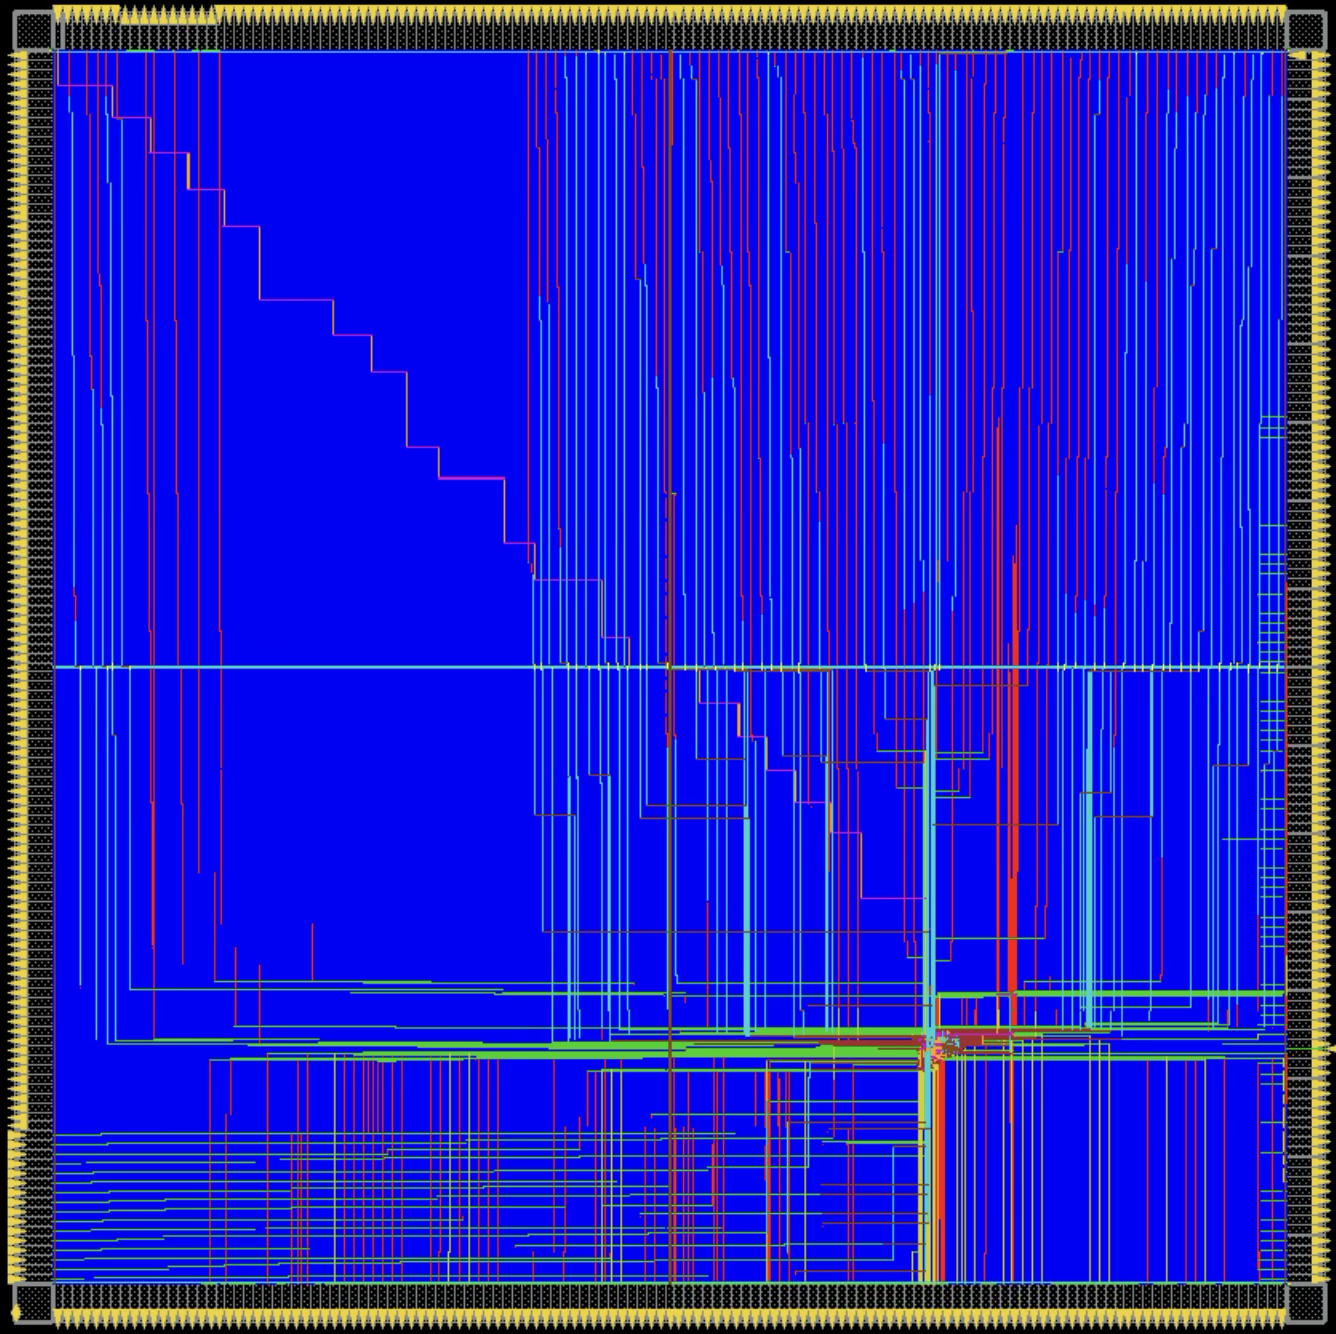
\includegraphics[width=0.8\textwidth]{assets/fig8_1_full_chip.png}
    \caption{Full Chip View}
\end{figure}

Στην απεικόνιση του πλήρους chip, διακρίνονται καθαρά οι κίτρινοι ακροδέκτες (bond pads) στην περιφέρεια, οι οποίοι σχηματίζουν το πλαίσιο επικοινωνίας με το εξωτερικό περιβάλλον. Είναι εμφανής η τεράστια διαφορά μεγέθους μεταξύ του πυρήνα (core logic), που βρίσκεται στο κέντρο, και του συνολικού εμβαδού που καταλαμβάνουν τα pads. Η εικόνα επιβεβαιώνει οπτικά ότι πρόκειται για μια σχεδίαση "Pad Limited", όπου οι διαστάσεις του chip καθορίζονται αποκλειστικά από τον αριθμό των απαιτούμενων ακροδεκτών και όχι από το μέγεθος της λογικής του κυκλώματος.

\begin{figure}[H]
    \centering
    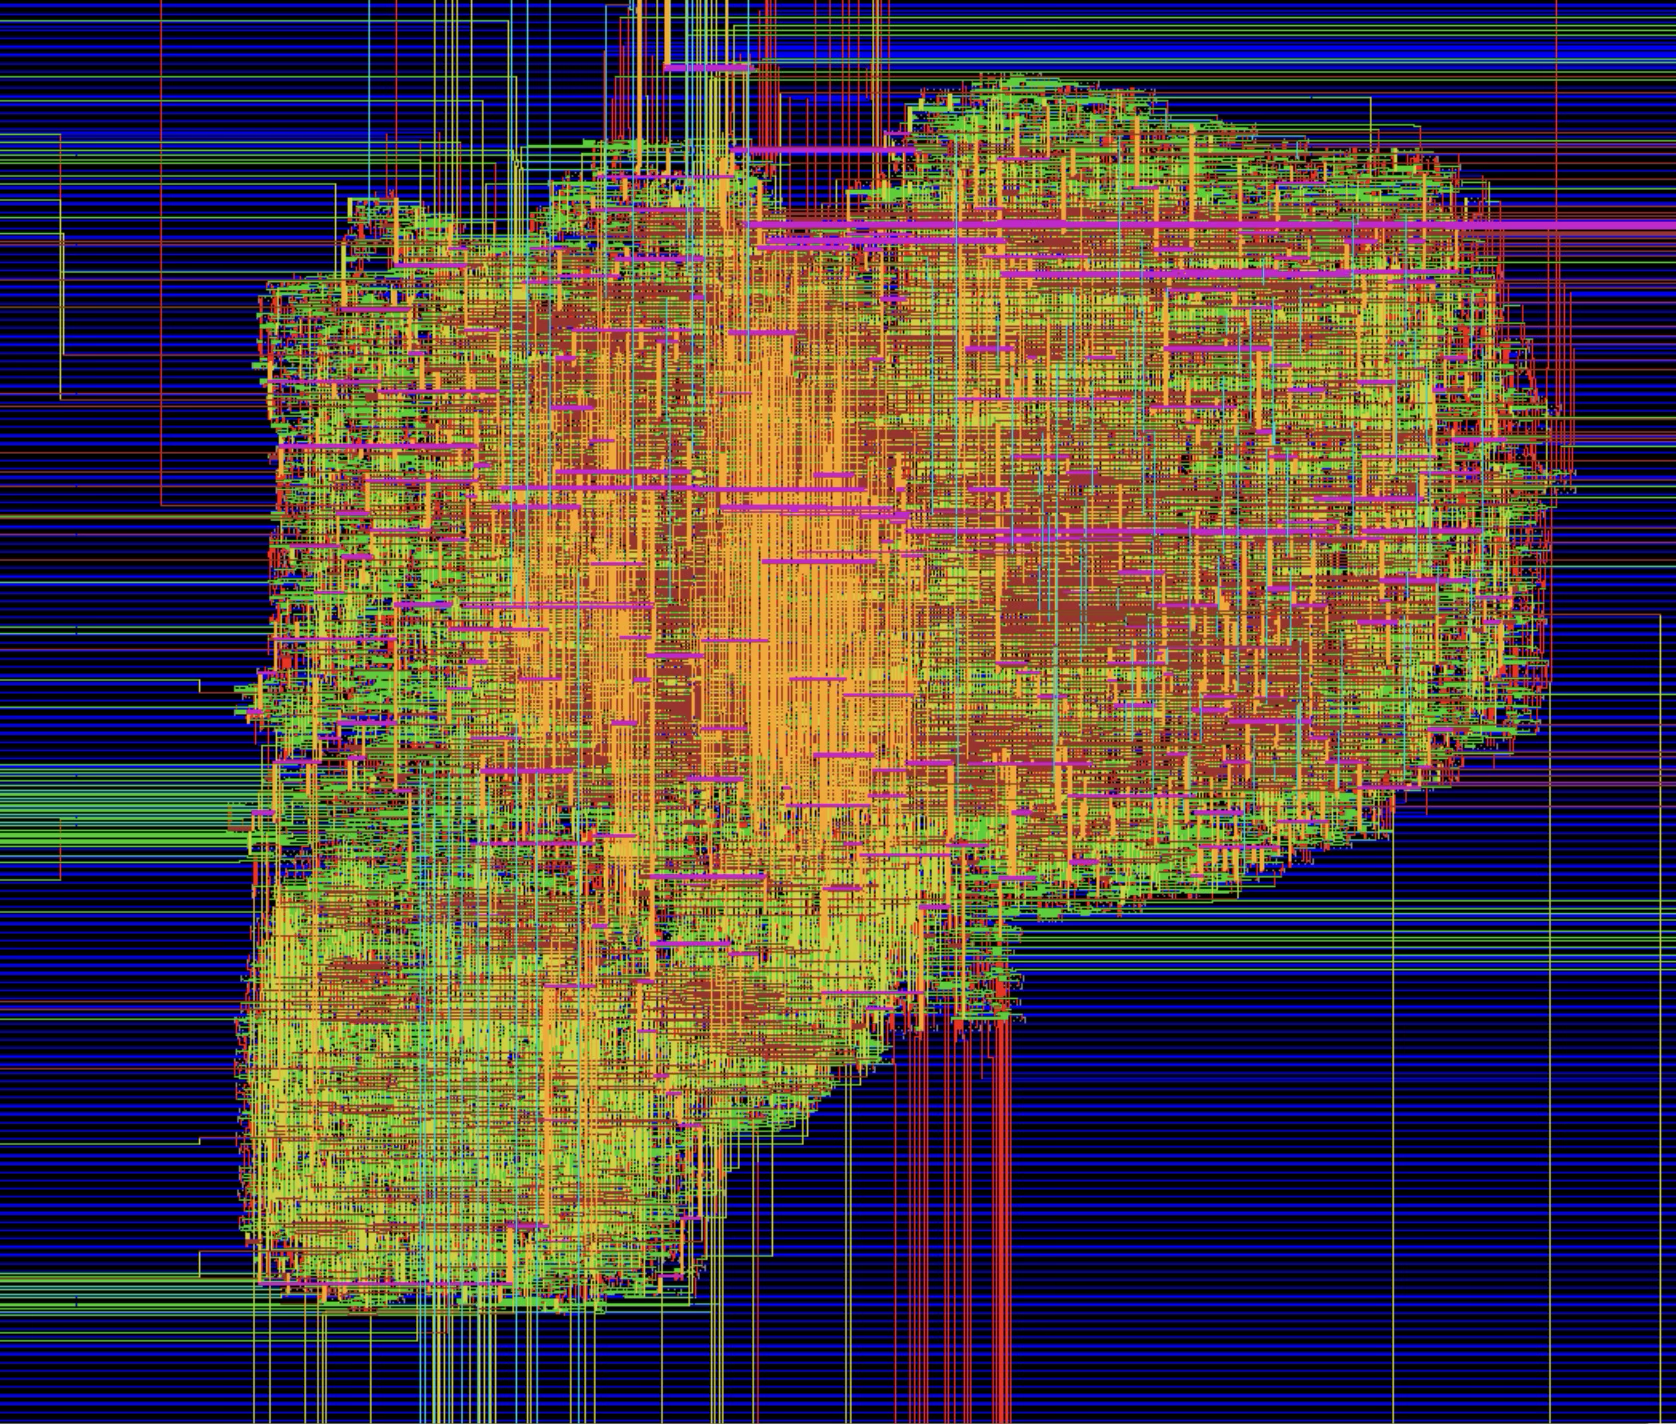
\includegraphics[width=0.8\textwidth]{assets/fig8_2_routing.png}
    \caption{Routed Interconnects}
\end{figure}

Η δεύτερη εικόνα εστιάζει στη δρομολόγηση των σημάτων από τον πυρήνα προς τους ακροδέκτες. Διακρίνονται τα μακριά καλώδια (long interconnects) που απαιτούνται για να συνδέσουν τα ports του μικρού πυρήνα με τα αντίστοιχα I/O cells στην περιφέρεια. Αυτές οι μεγάλες αποστάσεις δρομολόγησης, σε συνδυασμό με την καθυστέρηση των ίδιων των IO cells, εξηγούν τις σημαντικές παραβιάσεις χρονισμού (Setup violations) που παρατηρήθηκαν στα μονοπάτια Inputs-to-Registers (I2R) στον Πίνακα 8.2.

\begin{table}[H]
    \centering
    \caption{Total Area post Routing}
    \begin{tabular}{lr}
        \toprule
        Category & Area ($\mu m^2$) \\
        \midrule
        Άσκηση 1 & 34627.842 \\
        Άσκηση 8 & 7660571.274 \\
        \bottomrule
    \end{tabular}
\end{table}

Η συνολική επιφάνεια του chip εκτοξεύθηκε στα 7.660.571 $\mu m^2$, μια αύξηση της τάξης του $220\times$ σε σύγκριση με τον πυρήνα της Άσκησης 1 (34.627 $\mu m^2$). Αυτό το αποτέλεσμα είναι αναμενόμενο, καθώς τα κελιά εισόδου/εξόδου είναι φυσικά ογκώδη για να υποστηρίξουν τη μηχανική σύνδεση (wire bonding) και να αντέξουν τα ρεύματα οδήγησης, καθιστώντας τον πυρήνα (core) ένα ελάχιστο ποσοστό της συνολικής επιφάνειας του ολοκληρωμένου (Pad Limited Design).

\begin{table}[H]
    \centering
    \caption{Setup and Hold Slack post Routing}
    \begin{tabular}{lrrrr}
        \toprule
         & \multicolumn{2}{c}{\textbf{Άσκηση 1}} & \multicolumn{2}{c}{\textbf{Άσκηση 8}} \\
        \cmidrule(lr){2-3} \cmidrule(lr){4-5}
        Category & Setup Slack (ns) & Hold Slack (ns) & Setup Slack (ns) & Hold Slack (ns) \\
        \midrule
        I2O & - & - & - & - \\
        I2R & 2.531 & 0.241 & -5.880 & 1.760 \\
        R2O & 3.054 & 0.295 & 0.718 & 1.284 \\
        R2R & 1.452 & 0.032 & 1.400 & 0.032 \\
        \bottomrule
    \end{tabular}
\end{table}

Η συνολική κατανάλωση αυξήθηκε από τα 10,46 mW στα 292,3 mW. Όπως αποκαλύπτει ο Πίνακας 8.3, το 95,31\% αυτής της ενέργειας (278,6 mW) καταναλώνεται αποκλειστικά από τα I/Os (κατηγορία “IO”), λόγω των υψηλών τάσεων και των ρευμάτων που απαιτούνται για την οδήγηση των εξωτερικών χωρητικών φορτίων.

\begin{table}[H]
    \centering
    \caption{Power Consumption per Category post Routing}
    \resizebox{\textwidth}{!}{
    \begin{tabular}{lrrrrrrrrrr}
        \toprule
         & \multicolumn{5}{c}{\textbf{Άσκηση 1}} & \multicolumn{5}{c}{\textbf{Άσκηση 8}} \\
        \cmidrule(lr){2-6} \cmidrule(lr){7-11}
        Category & Leakage (mW) & Internal (mW) & Switching (mW) & Total (mW) & Row \% & Leakage (mW) & Internal (mW) & Switching (mW) & Total (mW) & Row \% \\
        \midrule
        Sequential & $1.93\times10^{-3}$ & 3.537 & 0.452 & 3.991 & 38.15 & $1.97\times10^{-3}$ & 3.49 & 1.824 & 5.319 & 1.82 \\
        Combinational & $2.38\times10^{-3}$ & 1.513 & 3.863 & 5.379 & 51.43 & $4.04\times10^{-3}$ & 1.95 & 3.94 & 5.897 & 2.017 \\
        Clock (Comb) & $4.81\times10^{-5}$ & 0.232 & 0.858 & 1.09 & 10.42 & $0.12\times10^{-3}$ & 0.59 & 1.91 & 2.492 & 0.852 \\
        IO & 0 & 0 & 0 & 0 & 0 & 28.86 & 247.1 & 2.68 & 278.6 & 95.31 \\
        Total & $4.355\times10^{-3}$ & 5.283 & 5.173 & 10.46 & 100 & 28.86 & 253.1 & 10.35 & 292.3 & 100 \\
        \bottomrule
    \end{tabular}}
\end{table}

Ενώ τα εσωτερικά μονοπάτια (R2R) διατήρησαν το θετικό τους slack (0,032 ns), παρατηρείται μεγάλη παραβίαση χρονισμού στα μονοπάτια εισόδου (I2R Setup Slack: -5,880 ns). Αυτή η αποτυχία οφείλεται στη σημαντική καθυστέρηση διάδοσης που εισάγουν τα κελιά εισόδου (input pads) σε συνδυασμό με την υψηλή συχνότητα των 250 MHz. Σε μια πραγματική σχεδίαση, αυτό θα απαιτούσε είτε χαλάρωση των περιορισμών χρονισμού για τις εισόδους, είτε χρήση ταχύτερων IO cells, είτε pipeline στα inputs για την αποκατάσταση του χρονισμού.
\newpage

\end{document}